% ============================================================================
%  COTALIA: Propuesta de servicios de agricultura de precisión · Etapa 01
%  Compilar con XeLaTeX:   latexmk -xelatex Cotalia_Etapa1.tex
%  Cifras del sitio: datos/datos_sitio.tex (generado por site_maps.py a partir de los datos de campo)
% ============================================================================
\documentclass[10pt]{article}

% ---------------------------------------------------------------- datos editables
\newcommand{\Empresa}{Cotalia}
\newcommand{\Equipo}{Tyrone Leslie, Jessie Anastasia Mvula, Carly Chery y Felix Wanjiku}
\newcommand{\Correo}{contacto@cotalia.cr}           % contacto ficticio: reemplazar si el equipo lo desea
\newcommand{\Web}{cotalia.cr}
\newcommand{\Direccion}{Campus Universidad EARTH, Las Mercedes de Guácimo, Limón, Costa Rica}
\newcommand{\Curso}{IGA-407 Agricultura de Precisión}
\newcommand{\Profesor}{Prof. Villalobos}
\newcommand{\Cliente}{Don Luis}
\newcommand{\ClienteCargo}{Encargado de la Finca Académica de Cultivos, Universidad EARTH}
\newcommand{\Fecha}{Septiembre de 2026}

% ============================================================================
%  COTALIA: sistema de diseño editorial
%  Tipografía: Inter (texto y titulares) + IBM Plex Mono (etiquetas, datos)
%  Paleta: tinta (verde casi negro), papel cálido, acento laterita (cobre)
% ============================================================================
\usepackage{fontspec}
\usepackage[spanish, es-noshorthands, es-tabla, es-nodecimaldot]{babel}
\usepackage[a4paper, top=27mm, bottom=26mm, inner=24mm, outer=24mm, headheight=12mm, headsep=9mm, footskip=12mm]{geometry}
\usepackage{xcolor}
\usepackage{graphicx}
\usepackage{tikz}
\usetikzlibrary{positioning, arrows.meta, calc, backgrounds}
\usepackage{pgfgantt}
\usepackage{booktabs, tabularx, array, multirow, colortbl, longtable}
\usepackage{catchfile}
\usepackage{enumitem}
\usepackage{caption}
\usepackage{float}
\usepackage{fancyhdr}
\usepackage[nobottomtitles*]{titlesec}
\usepackage{titletoc}
\usepackage{ragged2e}
\usepackage{lastpage}
\usepackage{qrcode}
\usepackage{microtype}
\usepackage{needspace}
\usepackage{etoolbox}
\usepackage[outline]{contour}
\contourlength{1.2pt}
\usepackage[hidelinks]{hyperref}
\def\UrlBreaks{\do\/}

% ---------------------------------------------------------------- paleta
\definecolor{tinta}{HTML}{0C1A17}       % casi negro, subtono verde
\definecolor{grafito}{HTML}{2E3834}     % texto
\definecolor{pizarra}{HTML}{717B77}     % texto secundario
\definecolor{linea}{HTML}{D8DBD6}       % filetes
\definecolor{niebla}{HTML}{F3F2EE}      % paneles
\definecolor{cobre}{HTML}{C4622D}       % acento: laterita
\definecolor{cobreclaro}{HTML}{E9A67F}
\definecolor{dosel}{HTML}{2F6B4F}       % verde secundario

% ---------------------------------------------------------------- tipografía
\setmainfont{Inter-Regular.otf}[BoldFont=Inter-SemiBold.otf, ItalicFont=Inter-Italic.otf,
  BoldItalicFont=Inter-SemiBoldItalic.otf, Scale=0.94, RawFeature=-calt]
\setmonofont{IBMPlexMono-Regular.otf}[BoldFont=IBMPlexMono-Medium.otf, Scale=0.94]
\newfontfamily\thin{Inter-Thin.otf}[RawFeature=-calt]
\newfontfamily\xlight{Inter-ExtraLight.otf}[RawFeature=-calt]
\newfontfamily\light{Inter-Light.otf}[RawFeature=-calt]
\newfontfamily\medium{Inter-Medium.otf}[RawFeature=-calt]
\newfontfamily\semi{Inter-SemiBold.otf}[RawFeature=-calt]
\newfontfamily\monomed{IBMPlexMono-Medium.otf}
\newfontfamily\monoreg{IBMPlexMono-Regular.otf}
\newcommand{\tnum}{\addfontfeature{Numbers=Monospaced}}

% ---------------------------------------------------------------- matemáticas (Fira Math, sans, a juego con Inter)
\usepackage{mathtools}
\usepackage{unicode-math}
\setmathfont{FiraMath-Regular.otf}[Scale=0.94]
% número con coma decimal dentro de fórmulas: 0,25 -> 0{,}25 (sin espacio de puntuación tras la coma)
\ExplSyntaxOn
\NewDocumentCommand{\mnum}{m}{ \tl_set:Ne \l_tmpa_tl {#1} \tl_replace_all:Nnn \l_tmpa_tl {,} {{,}} \tl_use:N \l_tmpa_tl }
\ExplSyntaxOff
% fórmulas tras una línea corta: mismo espacio que tras una línea larga
\makeatletter
\g@addto@macro\normalsize{\setlength\abovedisplayshortskip{\abovedisplayskip}\setlength\belowdisplayshortskip{\belowdisplayskip}}
\makeatother
\newtagform{cotalia}{\monoreg\fontsize{7.6}{9}\selectfont\color{pizarra}(}{)}
\usetagform{cotalia}
\setlength{\jot}{6pt}

% ---------------------------------------------------------------- logotipos de la tecnología usada
\linespread{1.32}
\setlength{\parskip}{0.55em}
\setlength{\parindent}{0pt}
\AtBeginDocument{\color{grafito}}
\frenchspacing
\AtBeginDocument{\RaggedRight}
\setlength{\emergencystretch}{2.5em}
\renewcommand{\bottomtitlespace}{0.18\textheight}

% etiqueta superior (eyebrow): mono, mayúsculas, espaciada
\newcommand{\eyebrow}[2][cobre]{\leavevmode{\hyphenpenalty=10000\monomed\fontsize{6.8}{9}\selectfont\addfontfeature{LetterSpace=14}\color{#1}\MakeUppercase{#2}}}
\newcommand{\lede}[1]{\leavevmode{\light\fontsize{13.2}{19.8}\linespread{1}\selectfont\raggedright\hyphenpenalty=10000\exhyphenpenalty=10000\color{tinta}#1\par}\vspace{0.7em}}
\newcommand{\datos}[1]{{\monoreg\small#1}}

% ---------------------------------------------------------------- numeración 01, 02...
\makeatletter
\renewcommand{\thesection}{\two@digits{\value{section}}}
\renewcommand{\thesubsection}{\thesection.\arabic{subsection}}
\renewcommand{\thefigure}{\two@digits{\value{figure}}}
\renewcommand{\thetable}{\two@digits{\value{table}}}
\renewcommand{\theequation}{\two@digits{\value{equation}}}
\newcommand{\numpag}{\two@digits{\value{page}}}
\newcommand{\indice}{\@starttoc{toc}}
\makeatother

% ---------------------------------------------------------------- títulos
\newcommand{\sectionbreak}{\clearpage}
\titleformat{\section}[display]
  {\normalfont}
  {\thin\fontsize{54}{54}\selectfont\color{cobre}\thesection}
  {6pt}
  {\xlight\fontsize{29}{34}\linespread{1}\selectfont\color{tinta}}
  [\vspace{2pt}{\color{linea}\rule{\linewidth}{0.4pt}}]
\titlespacing*{\section}{0pt}{-4pt}{12pt}
\titleformat{\subsection}[display]
  {\semi\fontsize{12.5}{16}\selectfont\color{tinta}}
  {\eyebrow{\thesubsection}}
  {3pt}
  {}
\titlespacing*{\subsection}{0pt}{16pt}{5pt}

% índice
\contentsmargin{0pt}
\makeatletter
\titlecontents{section}[2.6em]{\addvspace{7pt}}
  {\contentslabel[{\monomed\fontsize{8}{10}\selectfont\color{cobre}\thecontentslabel}]{2.6em}\medium\color{tinta}}
  {\hspace*{-2.6em}\medium\color{tinta}}
  {\hfill{\monoreg\small\color{pizarra}\two@digits{\thecontentspage}}}
  [\vspace{3pt}{\color{linea}\hrule height 0.3pt}]
\makeatother

% ---------------------------------------------------------------- logo (vectorial)
% Marca: tres curvas de nivel excéntricas y abiertas forman una "C"; el punto de cobre es la cota.
\newcommand{\CotaliaMarca}[3]{% #1 escala, #2 color del trazo, #3 color del punto
  \begin{tikzpicture}[scale=#1, line cap=round, baseline={(0,-0.32)}]
    \draw[#2, line width=#1*2.15pt] (0,0) ++(42:1) arc[start angle=42, end angle=318, radius=1];
    \draw[#2, line width=#1*2.15pt] (0.10,0.05) ++(48:0.70) arc[start angle=48, end angle=312, radius=0.70];
    \draw[#2, line width=#1*2.15pt] (0.19,0.10) ++(58:0.40) arc[start angle=58, end angle=302, radius=0.40];
    \fill[#3] (0.27,0.14) circle (0.135);
  \end{tikzpicture}}
\newcommand{\CotaliaLogo}[3]{% #1 escala, #2 color, #3 color del punto
  \mbox{\CotaliaMarca{#1}{#2}{#3}\hspace{\fpeval{#1*0.42}cm}%
  {\semi\fontsize{\fpeval{#1*26}}{\fpeval{#1*26}}\selectfont\addfontfeature{LetterSpace=-2.5}\color{#2}cotalia}}}

% ---------------------------------------------------------------- encabezado y pie
\pagestyle{fancy}
\fancyhf{}
\renewcommand{\headrulewidth}{0pt}
\fancyhead[L]{\raisebox{-1pt}{\CotaliaMarca{0.13}{tinta}{cobre}}\hspace{5pt}{\semi\fontsize{8.5}{10}\selectfont\color{tinta}\addfontfeature{LetterSpace=-1}cotalia}}
\fancyhead[R]{\eyebrow[pizarra]{Etapa 01 \,/\, Propuesta de servicios}}
\fancyfoot[L]{\eyebrow[pizarra]{Finca Académica EARTH \,/\, Lote de cultivo \AreaHa~ha}}
\fancyfoot[R]{{\monomed\fontsize{7.5}{9}\selectfont\color{tinta}\numpag}{\monoreg\fontsize{7.5}{9}\selectfont\color{pizarra}\,/\,\pageref{LastPage}}}
\fancypagestyle{plain}{}

% ---------------------------------------------------------------- tablas, listas, leyendas
\newcommand{\cab}[1]{\leavevmode{\monomed\fontsize{6.6}{8}\selectfont\addfontfeature{LetterSpace=10}\color{pizarra}#1}}
\newcolumntype{L}[1]{>{\raggedright\arraybackslash}p{#1}}
\newcolumntype{C}[1]{>{\centering\arraybackslash}p{#1}}
\newcolumntype{Y}{>{\raggedright\arraybackslash}X}
\renewcommand{\arraystretch}{1.5}
\AtBeginEnvironment{table}{\fontsize{8.9}{12.4}\linespread{1}\selectfont}
\setlength{\heavyrulewidth}{0.7pt}
\setlength{\lightrulewidth}{0.3pt}
\setlength{\cmidrulewidth}{0.3pt}
\setlength{\aboverulesep}{0pt}
\setlength{\belowrulesep}{0pt}
\newcommand{\filete}{\arrayrulecolor{linea}\midrule\arrayrulecolor{tinta}}

\setlist[itemize]{label={\color{cobre}\rule[0.28em]{0.55em}{0.7pt}}, leftmargin=1.5em, itemsep=0.25em, topsep=0.3em}
\setlist[enumerate]{label={\monomed\small\color{cobre}0\arabic*}, leftmargin=2.2em, itemsep=0.35em, topsep=0.3em}

\DeclareCaptionFont{capetq}{\monomed\fontsize{6.8}{9}\selectfont\addfontfeature{LetterSpace=12}\color{cobre}}
\DeclareCaptionFont{captxt}{\fontsize{8.3}{12.2}\linespread{1}\selectfont\color{pizarra}}
\DeclareCaptionLabelFormat{mayus}{\MakeUppercase{#1}~#2}
\captionsetup{labelfont=capetq, textfont=captxt, labelformat=mayus, labelsep=quad,
  justification=raggedright, singlelinecheck=false, skip=8pt}
\captionsetup[figure]{name=Fig.}
\captionsetup[table]{name=Tabla, position=top, skip=6pt}

% tarjeta de cifra clave
\newcommand{\cifra}[3]{% #1 valor, #2 unidad, #3 etiqueta
  \begin{minipage}[t]{\linewidth}
    {\color{tinta}\rule{\linewidth}{0.7pt}}\par\vspace{6pt}
    {\xlight\fontsize{30}{32}\linespread{1}\selectfont\color{tinta}#1}{\light\fontsize{12}{14}\selectfont\color{pizarra}\,#2}\par\vspace{4pt}
    \eyebrow[pizarra]{#3}
  \end{minipage}}

% celda de característica (rejilla de fortalezas)
\newcommand{\rasgo}[2]{%
  \begin{minipage}[t]{\linewidth}
    {\color{linea}\rule{\linewidth}{0.4pt}}\par\vspace{5pt}
    {\semi\color{tinta}#1}\par\vspace{2pt}
    {\fontsize{8.8}{13}\linespread{1}\selectfont #2}
  \end{minipage}}

% estado de un entregable: completado (círculo lleno), parcial (medio), pendiente (vacío)
\newcommand{\marcaC}{\tikz[baseline=-0.55ex]\fill[tinta] (0,0) circle (0.95mm);}
\newcommand{\marcaP}{\tikz[baseline=-0.55ex]{\fill[cobre] (0,-0.95mm) arc[start angle=-90, end angle=90, radius=0.95mm] -- cycle;
  \draw[cobre, line width=0.6pt] (0,0) circle (0.95mm);}}
\newcommand{\marcaN}{\tikz[baseline=-0.55ex]\draw[pizarra, line width=0.6pt] (0,0) circle (0.95mm);}
\newcommand{\estC}{\leavevmode\marcaC\hspace{4pt}{\semi\color{tinta}Completado}}
\newcommand{\estP}{\leavevmode\marcaP\hspace{4pt}{\semi\color{cobre}Parcial}}
\newcommand{\estN}{\leavevmode\marcaN\hspace{4pt}{\color{pizarra}Pendiente}}
\newcommand{\entregable}[2]{\leavevmode{\semi\color{tinta}#1}\par{\monoreg\fontsize{6.8}{9}\selectfont\color{pizarra}#2}}

% casilla de avance por entregable (tira de progreso)
\tikzset{celda/.style={minimum width=1.28cm, minimum height=0.95cm, inner sep=0pt, font=\monomed\fontsize{9}{10}\selectfont}}
\newcommand{\celda}[3]{% #1 x, #2 número, #3 estado C/P/N
  \ifx#3C\node[celda, fill=tinta, text=white] at (#1,0) {#2};\fi
  \ifx#3P\node[celda, draw=cobre, line width=0.6pt, text=cobre,
      path picture={\fill[cobre] (path picture bounding box.south west) rectangle ([yshift=0.16cm]path picture bounding box.south);}] at (#1,0) {#2};\fi
  \ifx#3N\node[celda, draw=linea, line width=0.6pt, text=pizarra] at (#1,0) {#2};\fi}

% globo en color para EGM2008 (modelo del geoide, sin logotipo propio)
\definecolor{globo}{HTML}{2F74B5}
\newcommand{\globoicono}{%
  \begin{tikzpicture}[baseline=0pt, x=1pt, y=1pt]
    \fill[globo] (12.5,12.5) circle (12.5);
    \begin{scope}
      \clip (12.5,12.5) circle (12.5);
      \foreach \rx in {4.5,9} {\draw[white, line width=0.55pt] (12.5,12.5) ellipse [x radius=\rx, y radius=12.5];}
      \draw[white, line width=0.55pt] (12.5,0) -- (12.5,25);
      \foreach \y in {5.5,12.5,19.5} {\draw[white, line width=0.55pt] (0,\y) -- (25,\y);}
    \end{scope}
    \draw[cobre, line width=1.4pt] (12.5,12.5) circle (12.5);
  \end{tikzpicture}}

% tarjeta de tecnología: logotipo, nombre, versión y función
\newcommand{\pila}[4]{%
  \begin{minipage}[t]{\linewidth}
    \setlength{\parskip}{0pt}%
    {\color{linea}\rule{\linewidth}{0.4pt}}\par\vspace{10pt}
    {\color{tinta}\fontsize{25}{25}\selectfont\raisebox{0pt}[26pt][2pt]{#1}}\par\vspace{8pt}
    {\semi\color{tinta}#2}\hspace{5pt}{\monoreg\fontsize{7}{9}\selectfont\color{pizarra}#3}\par\vspace{3pt}
    {\fontsize{8.3}{12}\linespread{1}\selectfont #4}
  \end{minipage}}

% subtítulo menor dentro de una subsección: no queda solo al pie de la página
\newcommand{\subtema}[1]{\par\needspace{5\baselineskip}\eyebrow[pizarra]{#1}\par\vspace{2pt}}

% nota lateral
\newcommand{\nota}[1]{\leavevmode{\fontsize{8.3}{12.4}\linespread{1}\selectfont\color{pizarra}#1\par}}

\graphicspath{{../outputs/}{../}}

% Generado por site_maps.py a partir de los datos de campo; no editar a mano.
\newcommand{\AreaLote}{9 845}
\newcommand{\AreaHa}{0,98}
\newcommand{\Perimetro}{426,1}
\newcommand{\CentroE}{543974,9}
\newcommand{\CentroN}{1128832,2}
\newcommand{\CentroLat}{10° 12' 30,64" N}
\newcommand{\CentroLon}{83° 35' 55,02" O}
\newcommand{\CentroLatDec}{10.20851}
\newcommand{\CentroLonDec}{-83.59862}
\newcommand{\CentroLatDecCom}{10,20851}
\newcommand{\CentroLonDecCom}{−83,59862}
\newcommand{\ElevMin}{38,47}
\newcommand{\ElevMax}{39,93}
\newcommand{\Relieve}{1,46}
\newcommand{\GradPlano}{1,3}
\newcommand{\AzPlano}{7}
\newcommand{\PendMedia}{1,5}
\newcommand{\PendMax}{4,3}
\newcommand{\PendPnoventaycinco}{3,0}
\newcommand{\NPuntos}{139}
\newcommand{\NElev}{131}
\newcommand{\NMuestras}{8}
\newcommand{\RMSE}{8,0}
\newcommand{\Geoide}{11,42}
\newcommand{\ZonaUnoArea}{5 248}
\newcommand{\ZonaUnoPct}{53}
\newcommand{\ZonaDosArea}{4 596}
\newcommand{\ZonaDosPct}{47}
\newcommand{\ZonaUnoPend}{1,0}
\newcommand{\ZonaDosPend}{2,1}
\newcommand{\ZonaUnoElev}{38,82}
\newcommand{\ZonaDosElev}{39,25}
\newcommand{\NPropuestas}{0}
\newcommand{\NTotalMuestras}{8}
\newcommand{\DepArea}{357}
\newcommand{\DepProf}{5}
\newcommand{\DepVol}{11}
\newcommand{\NPuntosTotal}{143}
\newcommand{\NVertices}{4}
\newcommand{\HrmsMin}{1,1}
\newcommand{\HrmsMax}{1,5}
\newcommand{\VrmsMin}{1,8}
\newcommand{\VrmsMax}{2,8}
\newcommand{\PdopMax}{1,12}

% Generado por method_figures.py a partir de los datos de campo; no editar a mano.
\newcommand{\HoraInicio}{07:40}
\newcommand{\HoraFin}{09:50}
\newcommand{\HoraVertices}{07:40–07:47}
\newcommand{\HoraGrilla}{07:58–09:20}
\newcommand{\HoraMuestras}{09:32–09:50}
\newcommand{\DuracionLev}{2~h~10~min}
\newcommand{\Epocas}{5}
\newcommand{\NEpocasCinco}{142}
\newcommand{\Ocupacion}{7}
\newcommand{\SatUsoMin}{31}
\newcommand{\SatUsoMax}{41}
\newcommand{\SatRastMin}{38}
\newcommand{\SatRastMax}{46}
\newcommand{\PdopMin}{0,70}
\newcommand{\HdopMax}{0,46}
\newcommand{\VdopMax}{0,94}
\newcommand{\HrmsMed}{1,2}
\newcommand{\VrmsMed}{2,3}
\newcommand{\BaseMin}{5,6}
\newcommand{\BaseMax}{157}
\newcommand{\BaseMed}{77}
\newcommand{\InclMed}{2,6}
\newcommand{\InclMax}{9,3}
\newcommand{\Baston}{1,71}
\newcommand{\AlturaAnt}{1,778}
\newcommand{\EspMediana}{8,5}
\newcommand{\EspMin}{5,5}
\newcommand{\EspMax}{10,0}
\newcommand{\Densidad}{133}
\newcommand{\DensidadTotal}{141}
\newcommand{\BaseE}{544015,5}
\newcommand{\BaseN}{1128769,1}
\newcommand{\ZMedMin}{38,43}
\newcommand{\ZMedMax}{39,95}
\newcommand{\Suavizado}{100}
\newcommand{\MAE}{6,0}
\newcommand{\Sesgo}{+0,1}
\newcommand{\PNoventa}{12,2}
\newcommand{\NMASpct}{91}
\newcommand{\NSSDA}{15,6}
\newcommand{\RMSEdos}{7,97}
\newcommand{\RMSEajuste}{3,7}
\newcommand{\NHull}{124}
\newcommand{\NFuera}{15}
\newcommand{\MallaCeldas}{157 518}
\newcommand{\MallaFilas}{583}
\newcommand{\MallaCols}{660}
\newcommand{\PlanoBetaUno}{−0,15}
\newcommand{\PlanoBetaDos}{−1,25}
\newcommand{\ZoomImagen}{18}
\newcommand{\PixelImagen}{0,59}
\newcommand{\FechaImagen}{21 de noviembre de 2025}
\newcommand{\RMSELambdaCero}{8,5}
\newcommand{\RMSELambdaMil}{8,5}
\newcommand{\RMSETPSHull}{7,6}
\newcommand{\RMSETINHull}{8,0}
\newcommand{\RMSEIDWHull}{9,1}
\newcommand{\RMSECTHull}{9,2}

\hypersetup{pdftitle={Cotalia: Propuesta de servicios, Etapa 01}, pdfauthor={Cotalia}, pdfsubject={\Curso}, pdfcreator={Cotalia}, pdfproducer={Cotalia}}

\begin{document}

% ============================================================================ PORTADA
\begin{titlepage}
\thispagestyle{empty}
\begin{tikzpicture}[remember picture, overlay]
  \fill[tinta] (current page.south west) rectangle (current page.north east);
  % arte generativo: curvas de nivel reales del lote (cada 2 cm) y las 8 muestras de suelo
  \node[anchor=north, inner sep=0pt] at ([yshift=-5.2cm]current page.north)
    {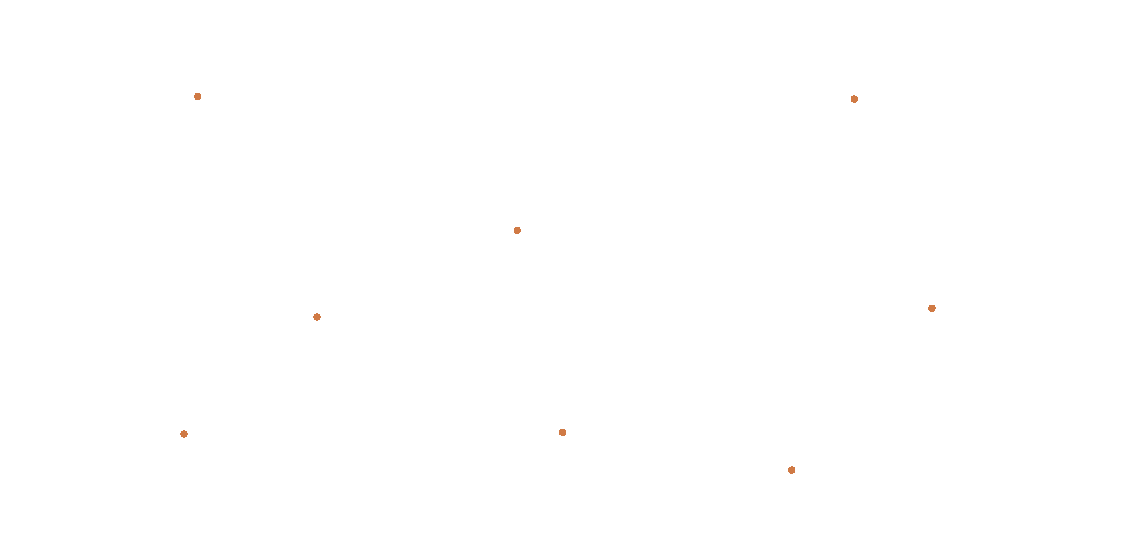
\includegraphics[width=18.6cm]{Informe_Etapa1/arte/portada_curvas.pdf}};
  % marca
  \node[anchor=north west, inner sep=0pt] at ([xshift=2.4cm, yshift=-2.2cm]current page.north west)
    {\CotaliaLogo{0.62}{white}{cobre}};
  \node[anchor=north east, inner sep=0pt] at ([xshift=-2.4cm, yshift=-2.55cm]current page.north east)
    {\eyebrow[cobreclaro]{Propuesta de servicios \,/\, Etapa 01}};
  % título (cada bloque en su propio nodo, con la fuente fijada en la opción font)
  \node[anchor=north west, inner sep=0pt] (ceja) at ([xshift=2.4cm, yshift=-15.3cm]current page.north west)
    {\eyebrow[cobreclaro]{Finca Académica de Cultivos \,·\, Universidad EARTH}};
  \node[anchor=north west, inner sep=0pt, text width=16.2cm, align=left, text=white,
        font=\xlight\fontsize{38}{43}\linespread{1}\selectfont] (titulo) at ([yshift=-0.55cm]ceja.south west)
    {Agricultura de precisión\\ para el manejo eficiente\\ del lote};
  \node[anchor=north west, inner sep=0pt, text width=16.2cm, align=left, text=white!72!tinta,
        font=\light\fontsize{12.5}{17}\linespread{1}\selectfont] at ([yshift=-0.55cm]titulo.south west)
    {Suelo, agua y nutrición: diagnóstico y plan para el lote de pasto de \AreaHa~ha en Las Mercedes de Guácimo, Limón.};
  % ficha inferior
  \draw[white!25!tinta, line width=0.4pt] ([xshift=2.4cm, yshift=4.1cm]current page.south west) -- ([xshift=-2.4cm, yshift=4.1cm]current page.south east);
  \node[anchor=north west, inner sep=0pt] at ([xshift=2.4cm, yshift=3.7cm]current page.south west) {%
    \renewcommand{\arraystretch}{1}\hyphenpenalty=10000\exhyphenpenalty=10000
    \begin{tabular}{@{}>{\raggedright\arraybackslash}p{4.3cm}>{\raggedright\arraybackslash}p{5.5cm}>{\raggedright\arraybackslash}p{2.8cm}>{\raggedright\arraybackslash}p{3.1cm}@{}}
      \eyebrow[cobreclaro]{Cliente} & \eyebrow[cobreclaro]{Equipo} & \eyebrow[cobreclaro]{Curso} & \eyebrow[cobreclaro]{Fecha} \\[7pt]
      {\fontsize{8.6}{12}\selectfont\color{white}\Cliente\par\color{white!60!tinta}Finca Académica de Cultivos, EARTH} &
      {\fontsize{8.6}{12}\selectfont\color{white}Tyrone Leslie · Jessie Anastasia Mvula\par Carly Chery · Felix Wanjiku} &
      {\fontsize{8.6}{12}\selectfont\color{white}IGA-407\par\color{white!60!tinta}\Profesor} &
      {\fontsize{8.6}{12}\selectfont\color{white}\Fecha} \\
    \end{tabular}};
\end{tikzpicture}
\end{titlepage}

% ============================================================================ RESUMEN
\thispagestyle{fancy}
\eyebrow{Resumen ejecutivo}\par\vspace{10pt}
{\xlight\fontsize{27}{32}\linespread{1}\selectfont\color{tinta}Del dato de campo\\a la decisión de manejo.\par}
\vspace{16pt}
\lede{\Empresa\ propone a la Finca Académica de Cultivos de la Universidad EARTH un servicio de agricultura de
precisión para manejar de forma eficiente el lote de pasto que se desea incorporar a la producción y la enseñanza
de cultivos: fertilización, pH, riego y drenaje decididos zona por zona.}
\vspace{6pt}
En esta primera etapa levantamos el lote con RTK-GNSS, validamos los datos, construimos su base
cartográfica (ubicación, polígono, curvas de nivel, pendientes y humedad topográfica), definimos dos zonas de manejo
provisionales y tomamos ocho muestras de suelo georreferenciadas, que ya están en el laboratorio. El terreno es casi plano,
con \Relieve~m de relieve y un gradiente general de \GradPlano~\% hacia el norte, y el manejo del agua es la prioridad:
el sector norte concentra el escurrimiento y presenta una posible zona de encharcamiento.

Este informe recoge el avance a la semana 4 del curso. De los once entregables oficiales, dos están completos
(mapa del campo y mapa de muestreo) y seis tienen avance parcial. Con los resultados de laboratorio, las pruebas de
campo y el análisis por zona entregaremos el plan de fertilización, encalado, riego y drenaje antes de la
presentación final de la semana 13.

\vspace{22pt}
\noindent
\begin{minipage}[t]{0.225\linewidth}\cifra{\AreaHa}{ha}{Área del lote}\end{minipage}\hfill
\begin{minipage}[t]{0.225\linewidth}\cifra{\NPuntosTotal}{pts}{Puntos RTK-GNSS}\end{minipage}\hfill
\begin{minipage}[t]{0.225\linewidth}\cifra{8}{/ 11}{Con avance}\end{minipage}\hfill
\begin{minipage}[t]{0.225\linewidth}\cifra{\NTotalMuestras}{}{Muestras de suelo}\end{minipage}

\vspace{30pt}
\noindent
\begin{minipage}[t]{0.47\linewidth}
\eyebrow[pizarra]{Preparado para}\par\vspace{4pt}
{\semi\color{tinta}\Cliente}\\ \ClienteCargo
\end{minipage}\hfill
\begin{minipage}[t]{0.47\linewidth}
\eyebrow[pizarra]{Preparado por}\par\vspace{4pt}
{\semi\color{tinta}\Empresa}\\ \Equipo
\end{minipage}

\clearpage
\eyebrow{Contenido}\par\vspace{8pt}
{\xlight\fontsize{27}{32}\linespread{1}\selectfont\color{tinta}Índice\par}
\vspace{14pt}
{\color{linea}\hrule height 0.3pt}
{\setcounter{tocdepth}{1}\indice}

% ============================================================================ 01 EMPRESA
\section{Quiénes somos}

\lede{\Empresa\ es una empresa de agricultura de precisión para el manejo eficiente de fincas. Convertimos datos
del suelo, del agua y del terreno en decisiones concretas: cuánto fertilizar, cómo corregir el pH, cuándo regar y
dónde drenar, zona por zona.}

Somos un equipo formado en la Universidad EARTH. El nombre viene de \emph{cota}, el punto medido del terreno: para
nosotros, toda decisión de manejo parte de un dato medido en el campo, con su ubicación exacta.

\vspace{10pt}
\noindent
\begin{minipage}[t]{0.47\linewidth}
\eyebrow{Misión}\par\vspace{5pt}
{\light\fontsize{11.5}{16.5}\linespread{1}\selectfont\color{tinta}Ayudar a productores y fincas del trópico húmedo a producir
más con menos insumos, con planes de fertilización, manejo del pH, riego y drenaje basados en datos medidos.}
\end{minipage}\hfill
\begin{minipage}[t]{0.47\linewidth}
\eyebrow{Visión}\par\vspace{5pt}
{\light\fontsize{11.5}{16.5}\linespread{1}\selectfont\color{tinta}Ser en 2030 la referencia en agricultura de precisión para
pequeñas y medianas fincas del Caribe costarricense, reconocida por hacer más eficiente el uso de fertilizantes, agua y enmiendas.}
\end{minipage}

\subsection{Fortalezas}
\noindent
\begin{minipage}[t]{0.31\linewidth}\rasgo{Suelo, agua y nutrición}{Integramos fertilidad, pH, humedad, compactación e infiltración para decidir por zona.}\end{minipage}\hfill
\begin{minipage}[t]{0.31\linewidth}\rasgo{Decisiones por zona}{Dosis de fertilizante, cal y agua ajustadas a cada parte del lote, no una dosis única.}\end{minipage}\hfill
\begin{minipage}[t]{0.31\linewidth}\rasgo{Datos de campo precisos}{RTK-GNSS centimétrico, muestreo georreferenciado y laboratorio en un mismo sistema.}\end{minipage}

\vspace{12pt}\noindent
\begin{minipage}[t]{0.31\linewidth}\rasgo{Ciencia verificable}{Validación cruzada y estándares de exactitud; cada resultado se puede recalcular.}\end{minipage}\hfill
\begin{minipage}[t]{0.31\linewidth}\rasgo{Tecnología abierta}{Procesamiento con software libre, sin licencias costosas para el cliente.}\end{minipage}\hfill
\begin{minipage}[t]{0.31\linewidth}\rasgo{Trópico húmedo}{Formación agronómica en EARTH, en condiciones de alta precipitación.}\end{minipage}

\subsection{Lo que ofrecemos}
\begin{table}[H]
\caption{Servicios.}
\begin{tabularx}{\linewidth}{@{}L{4.1cm}YL{3.3cm}@{}}
\toprule
\cab{SERVICIO} & \cab{DESCRIPCIÓN} & \cab{PRODUCTO} \\ \midrule
\semi Plan de fertilización & Dosis de nutrientes por zona según el análisis de suelo y el cultivo, con opción de dosis variable. & Plan por zona \\ \filete
\semi Manejo del pH & Diagnóstico de la acidez y recomendación de encalado por zona. & Dosis de cal por zona \\ \filete
\semi Riego inteligente & Diseño y programación del riego según la humedad del suelo, sensores y la demanda del cultivo. & Plan de riego \\ \filete
\semi Drenaje & Identificación de zonas de encharcamiento y trazado de drenajes. & Mapa de drenaje \\ \filete
\semi Muestreo y mapas de suelo & Muestreo georreferenciado, análisis físico y químico y mapas de variabilidad. & Mapas de fertilidad \\ \filete
\semi Zonas de manejo & Zonas homogéneas del lote para manejar cada parte según sus necesidades. & Mapa y estadísticas \\ \filete
\semi Diagnóstico de campo & Levantamiento RTK-GNSS, curvas de nivel, pendientes y escurrimiento. & Mapas del campo \\ \filete
\semi Acompañamiento técnico & Seguimiento de la aplicación de las recomendaciones y capacitación del personal. & Visitas e informes \\
\bottomrule
\end{tabularx}
\end{table}

\vspace{6pt}
\noindent\begin{minipage}{\linewidth}
{\color{linea}\rule{\linewidth}{0.4pt}}\par\vspace{6pt}
\begin{tabular}{@{}p{2.6cm}l@{}}
\eyebrow[pizarra]{Contacto} & {\semi\color{tinta}\Empresa} \quad \datos{\Correo \quad · \quad \Web} \\
 & \Direccion \\
\end{tabular}
\end{minipage}

% ============================================================================ 02 CLIENTE
\section{El cliente y sus necesidades}

\lede{Nuestro cliente es \Cliente, \ClienteCargo. La finca combina producción y enseñanza: sus lotes sirven para
prácticas de estudiantes, ensayos y producción de cultivos.}

El lote de estudio, hoy cubierto de pasto, se quiere preparar para producir cultivos. Para hacerlo de forma
eficiente hay que conocer antes su terreno, su suelo y cómo se mueve el agua, y traducirlo en un plan de
fertilización, encalado, riego y drenaje.

\subsection{Situación actual del lote}
\begin{itemize}
  \item Lote casi rectangular de \AreaLote~m² (\AreaHa~ha) y \Perimetro~m de perímetro, cubierto de pasto (imagen de noviembre de 2025).
  \item Terreno casi plano: según la superficie interpolada, de \ElevMin\ a \ElevMax~m\,s.\,n.\,m. aproximados, con \Relieve~m de relieve y un gradiente general de \GradPlano~\% hacia el norte.
  \item Trópico húmedo del Caribe costarricense, con lluvias abundantes casi todo el año: el exceso de agua es el principal factor de manejo.
  \item Colinda con un camino de acceso al noreste, un lote de pasto al norte y vegetación arbórea al suroeste.
\end{itemize}

\needspace{22\baselineskip}
\subsection{Necesidades identificadas}
A partir de la visita al lote y de los objetivos de la finca, identificamos siete necesidades:

\begin{table}[H]
\caption{Necesidades del cliente y respuesta de \Empresa.}
\begin{tabularx}{\linewidth}{@{}C{0.8cm}L{5.6cm}Y@{}}
\toprule
\cab{N.º} & \cab{NECESIDAD} & \cab{RESPUESTA} \\ \midrule
\leavevmode{\monomed\color{cobre}01} & Conocer el terreno y cómo se mueve el agua. & Mapa del campo: curvas de nivel, pendientes y escurrimiento (Sección~\ref{sec:analisis}). \\ \filete
\leavevmode{\monomed\color{cobre}02} & Evitar el encharcamiento y planificar el riego. & Humedad topográfica, depresiones, humedad e infiltración del suelo: base del drenaje y del riego inteligente. \\ \filete
\leavevmode{\monomed\color{cobre}03} & Conocer la fertilidad y el pH del suelo. & Análisis físico y químico de las muestras georreferenciadas y estado nutricional. \\ \filete
\leavevmode{\monomed\color{cobre}04} & Fertilizar y encalar de forma eficiente. & Plan de fertilización y dosis de cal por zona de manejo. \\ \filete
\leavevmode{\monomed\color{cobre}05} & Manejar de forma diferente las partes distintas del lote. & Zonas de manejo validadas con los datos de suelo. \\ \filete
\leavevmode{\monomed\color{cobre}06} & Preparar el lote antes de sembrar. & Recomendaciones de pre-siembra: labranza según la compactación, camas y drenajes. \\ \filete
\leavevmode{\monomed\color{cobre}07} & Contar con una base cartográfica para la enseñanza. & Polígono, vértices, área y mapas en CRTM05 (Sección~\ref{sec:sitio}). \\
\bottomrule
\end{tabularx}
\end{table}

% ============================================================================ 03 SITIO
\section{El sitio}\label{sec:sitio}

\lede{El lote está en la Finca Académica de la Universidad EARTH, en Las Mercedes de Guácimo, provincia de Limón,
sobre la llanura del Caribe de Costa Rica.}

\vspace{4pt}
\noindent
\begin{minipage}[c]{0.74\linewidth}
\renewcommand{\arraystretch}{1.5}
\begin{tabular}{@{}p{3.3cm}l@{}}
\eyebrow[pizarra]{Centroide · CRTM05} & \datos{E \CentroE~m \quad N \CentroN~m} \\
\eyebrow[pizarra]{Centroide · WGS 84} & \datos{\CentroLat \quad \CentroLon} \\
\eyebrow[pizarra]{Decimales} & \datos{\CentroLatDecCom;\ \CentroLonDecCom} \\
\eyebrow[pizarra]{Elevación} & \datos{\ElevMin–\ElevMax~m\,s.\,n.\,m. (superficie; EGM2008)} \\
\end{tabular}
\end{minipage}\hfill
\begin{minipage}[c]{0.2\linewidth}
\raggedleft
\edef\qrurl{https://www.openstreetmap.org/?mlat=\CentroLatDec\&mlon=\CentroLonDec\#map=17/\CentroLatDec/\CentroLonDec}%
{\color{tinta}\expandafter\qrcode\expandafter[\expandafter]\expandafter{\qrurl}}\\[3pt]
\eyebrow[pizarra]{Abrir ubicación}
\end{minipage}

\begin{figure}[H]
\centering
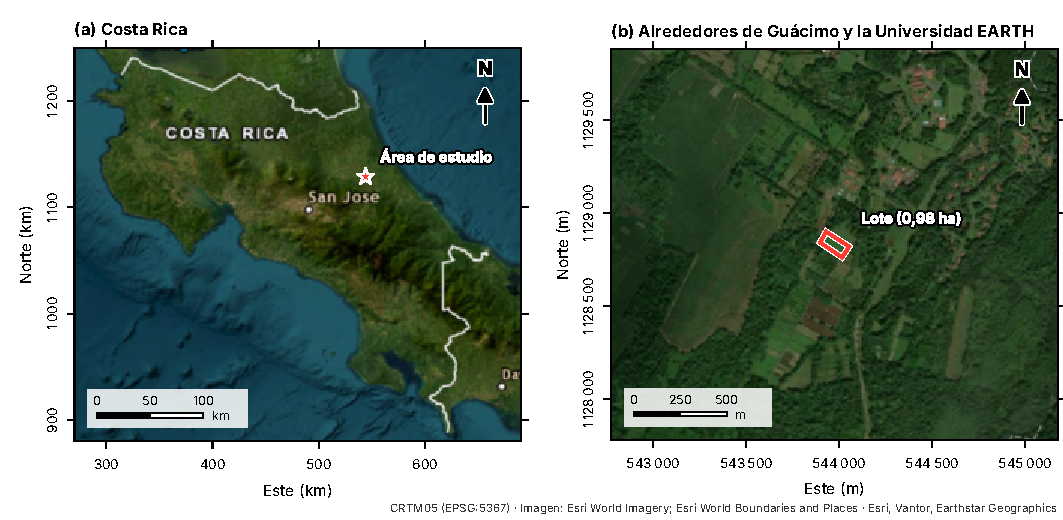
\includegraphics[width=\linewidth]{Figura_Ubicacion.pdf}
\caption{Ubicación del lote. (a) Costa Rica; la estrella marca el área de estudio. (b) Alrededores de Guácimo y la
Universidad EARTH, con el lote en rojo. Coordenadas CRTM05; la flecha indica el norte de cuadrícula, que difiere del
norte verdadero en 0,07°.}
\end{figure}

\clearpage
\subsection{Polígono y coordenadas}
El lote es un polígono de cuatro vértices levantados con RTK-GNSS: \AreaLote~m² (\AreaHa~ha) y \Perimetro~m de
perímetro. Sus ángulos internos están entre 87° y 94°, por lo que es casi un rectángulo orientado de noroeste a sureste.

\begin{figure}[H]
\centering
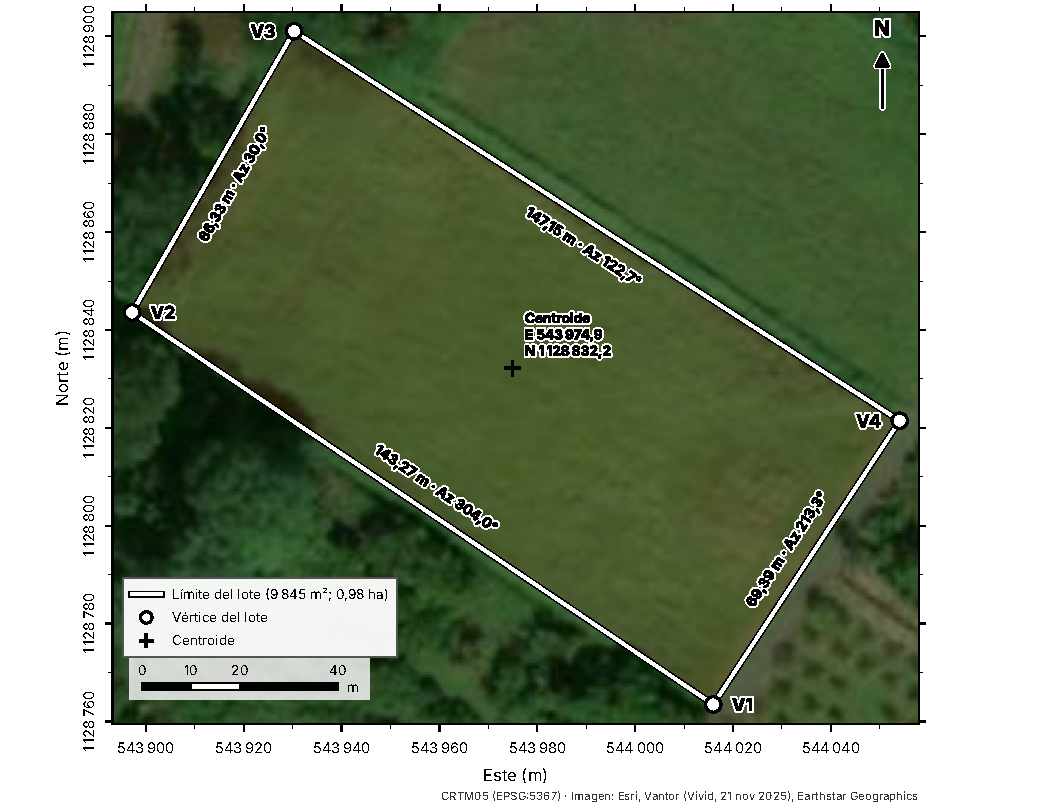
\includegraphics[width=0.78\linewidth]{Figura_Lote_Poligono.pdf}
\caption{Polígono del lote: vértices, longitud y azimut de cuadrícula de cada lado, y centroide. Coordenadas CRTM05 (EPSG:5367), la proyección transversal de Mercator oficial de Costa Rica; el área es la de la cuadrícula, ≈\,1,5~m² menor que sobre el terreno.}
\end{figure}

\begin{table}[H]
\caption{Vértices del lote en CRTM05 y WGS 84, elevación aproximada y ángulo interno.}
\small\tnum\renewcommand{\arraystretch}{1.22}
\begin{tabular*}{\linewidth}{@{\extracolsep{\fill}}lrrrrrr@{}}
\toprule
\cab{VÉRTICE} & \cab{ESTE (m)} & \cab{NORTE (m)} & \cab{LATITUD} & \cab{LONGITUD} & \cab{ELEV. (m)} & \cab{ÁNGULO} \\ \midrule
V1 & 544015,952 & 1128763,463 & 10° 12' 28,40" N & 83° 35' 53,68" O & 40,00 & 89,3\textdegree \\
V2 & 543897,174 & 1128843,573 & 10° 12' 31,01" N & 83° 35' 57,58" O & 39,20 & 94,0\textdegree \\
V3 & 543930,292 & 1128901,045 & 10° 12' 32,88" N & 83° 35' 56,49" O & 38,52 & 87,2\textdegree \\
V4 & 544054,059 & 1128821,450 & 10° 12' 30,28" N & 83° 35' 52,42" O & 38,98 & 89,4\textdegree \\
\bottomrule

\end{tabular*}
\end{table}

\begin{table}[H]
\caption{Lados del polígono: longitud, azimut de cuadrícula y rumbo.}
\small\tnum\renewcommand{\arraystretch}{1.22}
\begin{tabular*}{\linewidth}{@{\extracolsep{\fill}}lrrr@{}}
\toprule
\cab{LADO} & \cab{LONGITUD (m)} & \cab{AZIMUT} & \cab{RUMBO} \\ \midrule
V1--V2 & 143,27 & 304,00\textdegree & N 56° 00' O \\
V2--V3 & 66,33 & 29,95\textdegree & N 29° 57' E \\
V3--V4 & 147,15 & 122,75\textdegree & S 57° 15' E \\
V4--V1 & 69,39 & 213,31\textdegree & S 33° 19' O \\
\midrule
\textbf{Perímetro} & \textbf{426,14} & & \\
\bottomrule

\end{tabular*}
\end{table}


% ============================================================================ 04 ANÁLISIS
\section{Análisis}\label{sec:analisis}

\lede{Con los \NElev\ puntos de levantamiento y las \NMuestras\ muestras de suelo (\NPuntos\ puntos RTK-GNSS; los
vértices solo definen el límite) construimos una superficie de elevación validada, con un error de validación cruzada
de \RMSE~cm, y a partir de ella cinco productos. Cada uno responde a una necesidad del cliente; los métodos se
detallan en la Sección~\ref{sec:metodologia}.}

\vspace{14pt}
\eyebrow[pizarra]{El lote en cifras}\par\vspace{8pt}
\noindent
\begin{minipage}[t]{0.225\linewidth}\cifra{\Relieve}{m}{Relieve}\end{minipage}\hfill
\begin{minipage}[t]{0.225\linewidth}\cifra{\GradPlano}{\%}{Gradiente general}\end{minipage}\hfill
\begin{minipage}[t]{0.225\linewidth}\cifra{\PendMedia}{\%}{Pendiente media}\end{minipage}\hfill
\begin{minipage}[t]{0.225\linewidth}\cifra{2}{}{Zonas de manejo}\end{minipage}

\vspace{26pt}
\eyebrow[pizarra]{Productos}\par\vspace{6pt}
\begin{tabularx}{\linewidth}{@{}L{1.1cm}YL{3.6cm}@{}}
\arrayrulecolor{linea}\midrule\arrayrulecolor{tinta}
\leavevmode{\monomed\color{cobre}04.1} & Topografía: curvas de nivel cada 25~cm & \datos{Fig. 03} \\ \filete
\leavevmode{\monomed\color{cobre}04.2} & Pendientes y dirección de escurrimiento & \datos{Fig. 04} \\ \filete
\leavevmode{\monomed\color{cobre}04.3} & Humedad topográfica y depresiones & \datos{Fig. 05} \\ \filete
\leavevmode{\monomed\color{cobre}04.4} & Zonas de manejo provisionales & \datos{Fig. 06} \\ \filete
\leavevmode{\monomed\color{cobre}04.5} & Muestreo de suelos: 8 muestras georreferenciadas & \datos{Fig. 07} \\ \filete
\end{tabularx}

\clearpage
\subsection{Topografía}
Según la superficie interpolada, el lote desciende suavemente de sur a norte: de \ElevMax~m cerca de la esquina sur
(V1) a \ElevMin~m en el sector norte, junto a la muestra M2; en los puntos usados para la superficie, las elevaciones
medidas van de \ZMedMax\ a \ZMedMin~m. Las curvas cada 25~cm cumplen el estándar NMAS de exactitud para esta
superficie (Sección~\ref{sec:met-mde}). El borde
suroeste, hacia el bosque, es la parte más alta; el noreste, junto al camino, la más baja.

\begin{figure}[H]
\centering
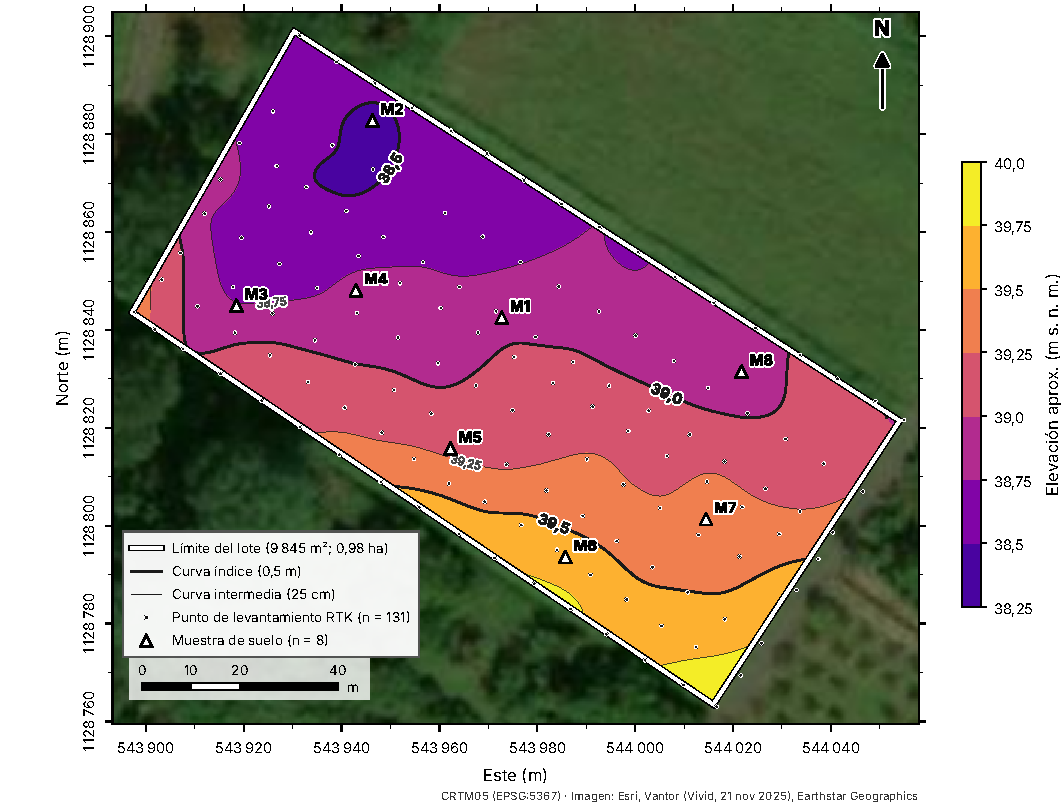
\includegraphics[width=\linewidth]{Figura_Curvas_de_Nivel.pdf}
\caption{Curvas de nivel cada 25~cm (índice cada 0,5~m). Elevación aproximada sobre el nivel del mar (EGM2008).}
\end{figure}

\clearpage
\subsection{Pendientes y escurrimiento}
La pendiente local media es de \PendMedia~\% (máxima \PendMax~\%; el 95~\% del lote queda por debajo de
\PendPnoventaycinco~\%): un terreno de plano a suavemente inclinado según las clases de FAO (2006, cuadro 7): tres cuartas partes del lote tienen menos de 2~\% y el resto, entre 2 y 5~\%. El riesgo de
erosión es bajo; el reto es evacuar el exceso de agua, que corre hacia el norte y el noreste.

\begin{figure}[H]
\centering
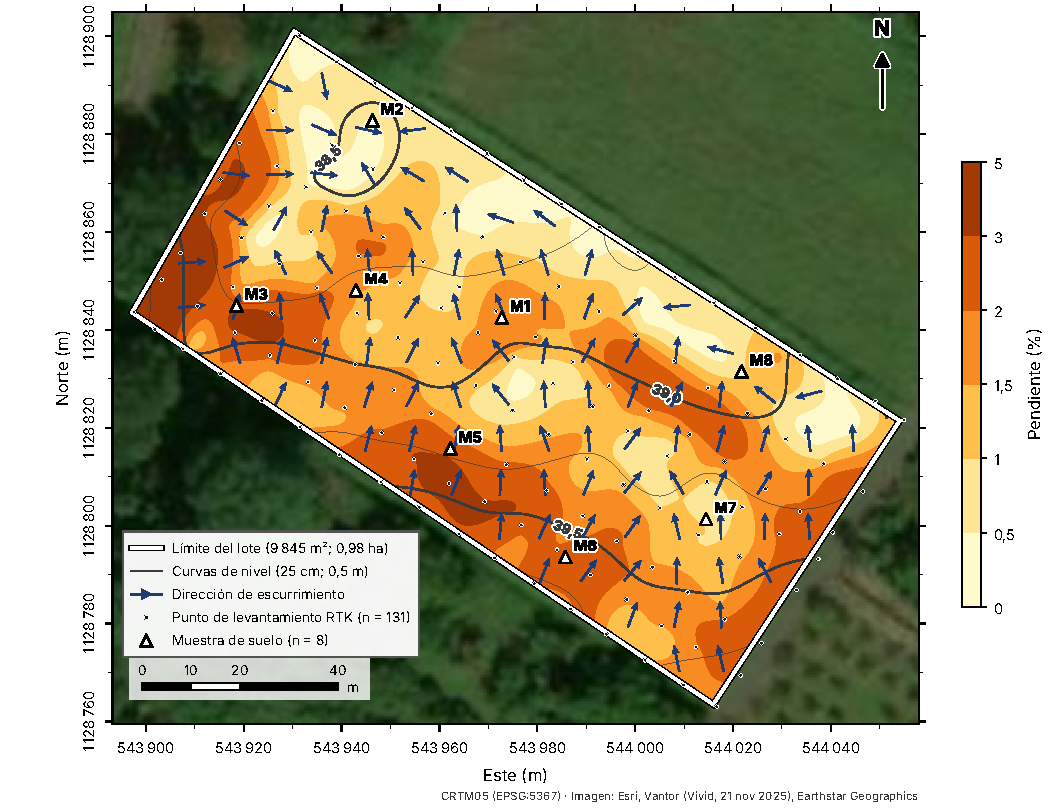
\includegraphics[width=\linewidth]{Figura_Pendientes.pdf}
\caption{Pendiente local y dirección de escurrimiento superficial.}
\end{figure}

\clearpage
\subsection{Humedad y drenaje}
El índice topográfico de humedad muestra dónde se concentra el agua. Varios cauces convergen hacia el sector de M2,
donde detectamos una \textbf{depresión potencial} de unos \DepArea~m², hasta \DepProf~cm de profundidad y
≈\,\DepVol~m³ de almacenamiento; otro cauce corre paralelo al borde noreste. Son las áreas prioritarias para
drenaje, y conviene verificarlas en el campo después de una lluvia fuerte.

\begin{figure}[H]
\centering
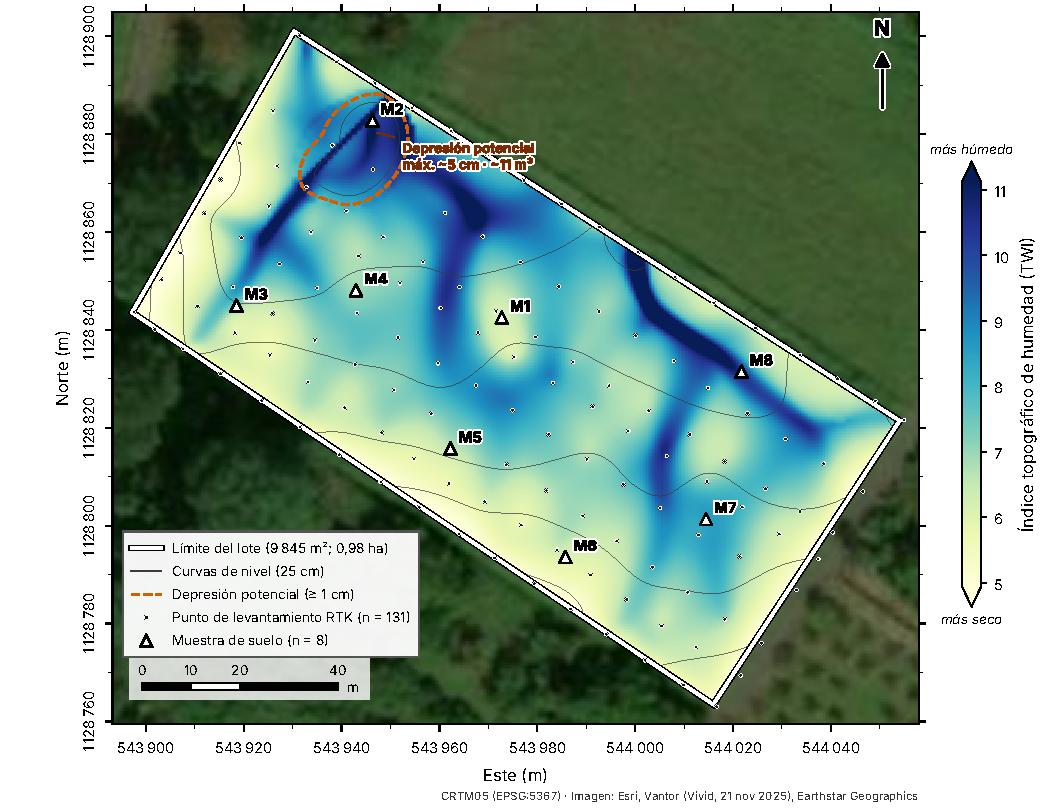
\includegraphics[width=\linewidth]{Figura_Humedad.pdf}
\caption{Índice topográfico de humedad (TWI) y depresión potencial (línea discontinua).}
\end{figure}

\clearpage
\subsection{Zonas de manejo}
Agrupamos el lote según elevación, pendiente y humedad con c-medias difuso; los índices FPI y NCE indican que dos
zonas describen mejor el terreno. Son \textbf{provisionales}: se basan solo en el terreno y deben confirmarse con
los análisis de suelo.

\vspace{4pt}\noindent
\begin{minipage}[t]{0.47\linewidth}
\cifra{\ZonaUnoPct}{\%}{Zona 1 · baja y húmeda}\par\vspace{4pt}
\nota{\ZonaUnoArea~m² · elevación media \ZonaUnoElev~m · pendiente \ZonaUnoPend~\%. Prioridad: drenaje.}
\end{minipage}\hfill
\begin{minipage}[t]{0.47\linewidth}
\cifra{\ZonaDosPct}{\%}{Zona 2 · alta y mejor drenada}\par\vspace{4pt}
\nota{\ZonaDosArea~m² · elevación media \ZonaDosElev~m · pendiente \ZonaDosPend~\%.}
\end{minipage}

\begin{figure}[H]
\centering
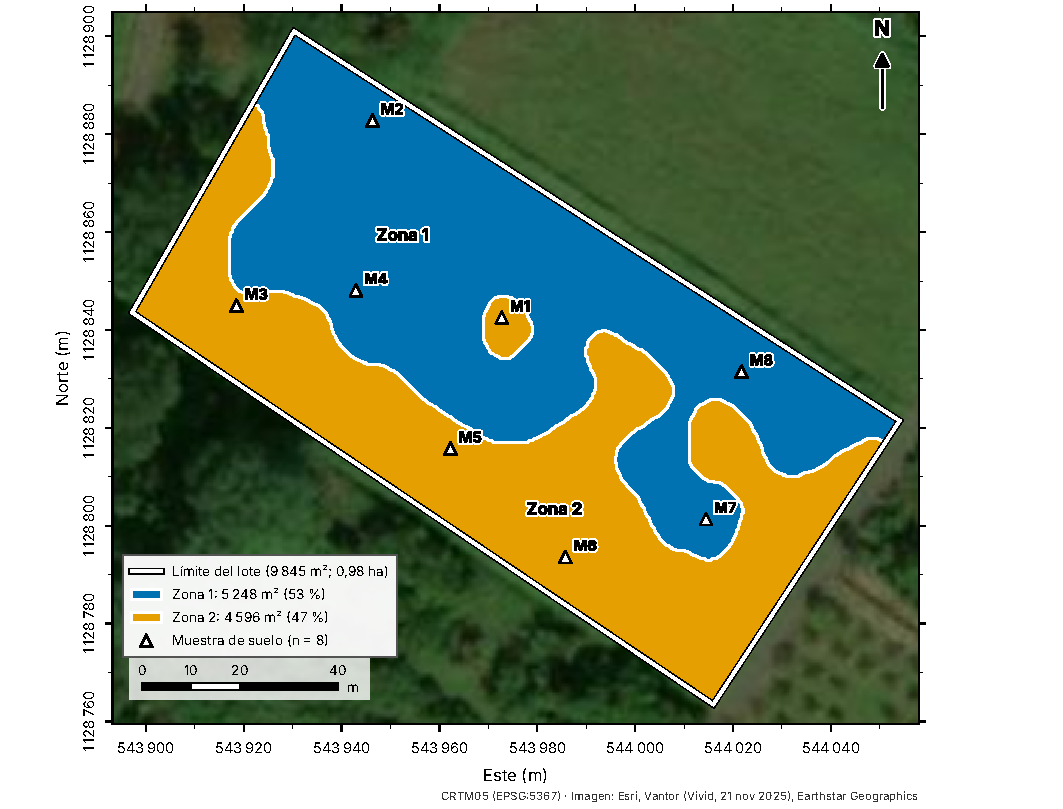
\includegraphics[width=0.92\linewidth]{Figura_Zonas_de_Manejo.pdf}
\caption{Zonas de manejo provisionales (c-medias difuso sobre elevación, pendiente y TWI).}
\end{figure}

\clearpage
\subsection{Muestreo de suelos}
El 26 de septiembre tomamos \NMuestras\ muestras de suelo en los puntos M1–M8, cuatro en cada zona de manejo, con
coordenadas RTK centimétricas. Las muestras están en el laboratorio para los análisis físico y químico. Con ocho
muestras no es posible un mapa geoestadístico (kriging); los mapas de las propiedades del suelo se apoyarán en las
zonas de manejo y en el terreno.

\begin{figure}[H]
\centering
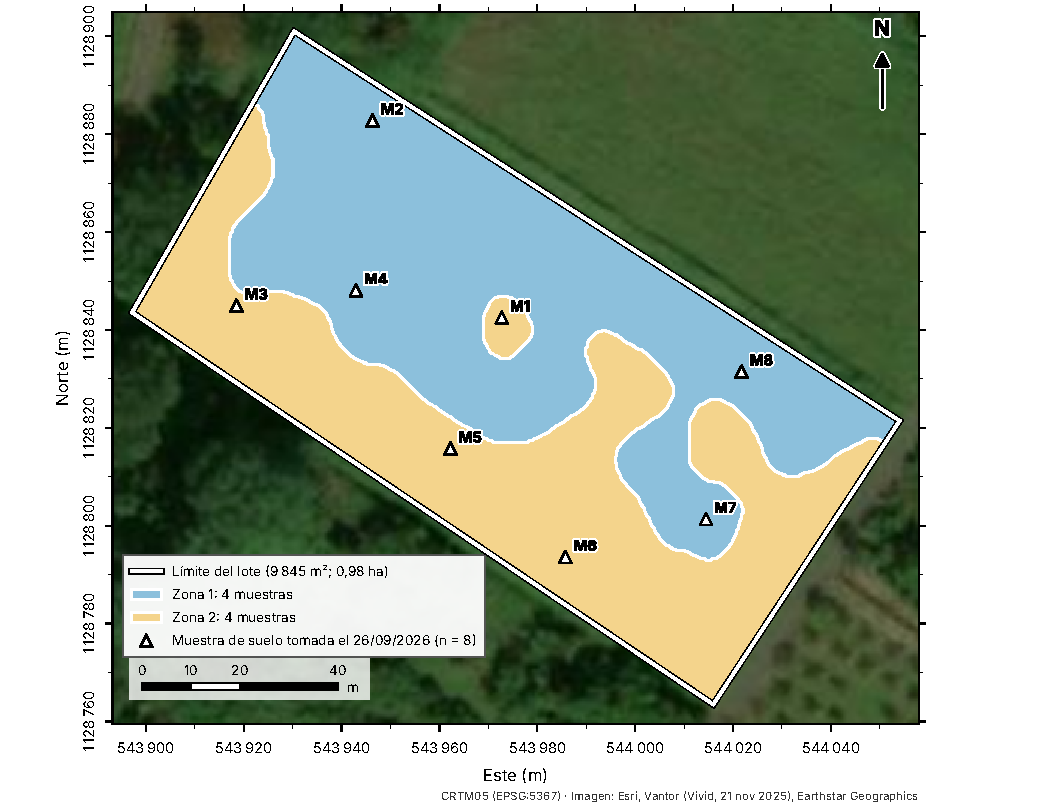
\includegraphics[width=\linewidth]{Figura_Plan_de_Muestreo.pdf}
\caption{Mapa de muestreo: 8 muestras de suelo tomadas el 26 de septiembre de 2026 (M1–M8), cuatro por zona.}
\end{figure}

\clearpage
\subsection{Recomendaciones preliminares}
\begin{enumerate}
  \item \textbf{Drenaje primero.} Drenaje superficial en la depresión del sector de M2 y a lo largo del borde noreste, hacia donde converge el agua.
  \item \textbf{Parcelas y camas.} Orientar camas y drenajes según el gradiente general, hacia el norte; con pendientes menores de 5~\% el riesgo de erosión es bajo.
  \item \textbf{Fertilización y pH por zona.} Con los análisis de laboratorio, calcular la dosis de cal y de fertilizante de cada zona, en lugar de una dosis única para todo el lote.
  \item \textbf{Riego y humedad.} Medir la humedad del suelo por zona para decidir si el cultivo necesitará riego en los periodos más secos y dónde instalar sensores.
  \item \textbf{Enseñanza.} Usar las dos zonas como contraste didáctico en las prácticas de estudiantes.
\end{enumerate}

\vspace{30pt}
{\color{linea}\rule{\linewidth}{0.4pt}}\par\vspace{8pt}
\eyebrow{Próximo paso}\par\vspace{6pt}
\lede{Semana 5: preparación de las pruebas de campo. Semana 6: humedad y compactación en los ocho puntos de muestreo
e infiltración en cuatro de ellos, dos por zona. Los resultados de laboratorio de M1–M8 se esperan entre las semanas
5 y 8.}

% ============================================================================ 05 METODOLOGÍA
\section{Metodología}\label{sec:metodologia}

\lede{El trabajo se organiza en tres fases y doce pasos: diagnóstico (semana 4, completado), campo y laboratorio
(semanas 4 a 8) y síntesis (semanas 9 a 13). Aquí explicamos el plan y, paso a paso, cómo medimos el lote y cómo
hicimos cada mapa.}

\begin{figure}[H]
\centering
\begin{tikzpicture}[
    paso/.style={rectangle, draw=tinta, line width=0.5pt, fill=tinta, text=white, text width=4.25cm,
                 minimum height=1.45cm, inner sep=6.5pt, align=left, font=\fontsize{8.6}{11}\linespread{1}\selectfont\semi,
                 execute at begin node={\hyphenpenalty=10000\exhyphenpenalty=10000}},
    futuro/.style={paso, fill=white, draw=linea, text=tinta},
    meta/.style={paso, fill=cobre, draw=cobre, text=white},
    flecha/.style={-{Stealth[length=2mm, width=1.5mm]}, line width=0.5pt, color=pizarra},
    node distance=0.32cm and 0.62cm]
  % fase 1
  \node[anchor=south west, inner sep=0pt] (h1) at (0,0.25) {\eyebrow{Fase 1 · Semana 4}};
  \node[paso, anchor=north west] (a1) at (0,0) {\eyebrow[cobreclaro]{Paso 01}\\ Levantamiento RTK-GNSS y muestras M1–M8};
  \node[paso, below=of a1] (a2) {\eyebrow[cobreclaro]{Paso 02}\\ Control de calidad de los datos};
  \node[paso, below=of a2] (a3) {\eyebrow[cobreclaro]{Paso 03 · E01}\\ Mapa del campo};
  \node[paso, below=of a3] (a4) {\eyebrow[cobreclaro]{Paso 04 · E02}\\ Zonas provisionales y mapa de muestreo};
  % fase 2
  \node[futuro, right=of a1] (b1) {\eyebrow{Paso 05 · E05 E06 E07}\\ Humedad, compactación e infiltración};
  \node[anchor=south west, inner sep=0pt] at (b1.north west |- h1.south west) {\eyebrow{Fase 2 · Semanas 4–8}};
  \node[futuro, below=of b1] (b2) {\eyebrow{Paso 06 · E03}\\ Análisis físico en laboratorio};
  \node[futuro, below=of b2] (b3) {\eyebrow{Paso 07 · E04}\\ Análisis químico en laboratorio};
  \node[futuro, below=of b3] (b4) {\eyebrow{Paso 08}\\ Base de datos de suelo por zona};
  % fase 3
  \node[futuro, right=of b1] (c1) {\eyebrow{Paso 09 · E08}\\ Estado nutricional};
  \node[anchor=south west, inner sep=0pt] at (c1.north west |- h1.south west) {\eyebrow{Fase 3 · Semanas 9–13}};
  \node[futuro, below=of c1] (c2) {\eyebrow{Paso 10 · E09}\\ Mapas de variabilidad espacial};
  \node[futuro, below=of c2] (c3) {\eyebrow{Paso 11 · E10}\\ Zonas de manejo definitivas};
  \node[futuro, below=of c3] (c4) {\eyebrow{Paso 12 · E11}\\ Recomendaciones de pre-siembra};
  \node[meta, below=of c4] (c5) {\eyebrow[white]{Semanas 12 y 13}\\ Informe final y presentación};
  \foreach \x in {a,b,c} {\draw[flecha] (\x1) -- (\x2); \draw[flecha] (\x2) -- (\x3); \draw[flecha] (\x3) -- (\x4);}
  \draw[flecha] (c4) -- (c5);
  \draw[flecha] (a4.east) -- ++(0.31,0) |- (b1.west);
  \draw[flecha] (b4.east) -- ++(0.31,0) |- (c1.west);
  \node[anchor=north west] at ($(a4.south west)+(0,-0.35)$)
    {\tikz\fill[tinta] (0,0) rectangle (0.32,0.2);\ \eyebrow[pizarra]{Completado}\qquad
     \tikz\draw[linea, line width=0.6pt] (0,0) rectangle (0.32,0.2);\ \eyebrow[pizarra]{Por realizar}\qquad
     \eyebrow[pizarra]{E01–E11: entregables}};
\end{tikzpicture}
\caption{Flujo de trabajo en tres fases. Los pasos que generan un entregable oficial lo indican (E01 a E11).}
\end{figure}

\begin{table}[H]
\caption{Pasos, métodos y productos. Los métodos de la fase 1 se detallan en las Secciones \ref{sec:met-campo} a \ref{sec:met-carto}.}
\label{tab:pasos}
\renewcommand{\arraystretch}{1.36}
\begin{tabularx}{\linewidth}{@{}>{\raggedright\arraybackslash\hyphenpenalty=10000\exhyphenpenalty=10000}p{3.35cm}YL{2.9cm}@{}}
\toprule
\cab{PASO} & \cab{MÉTODO} & \cab{PRODUCTO} \\ \midrule
\multicolumn{3}{@{}l}{\eyebrow{Fase 1 · Diagnóstico · Semana 4 · Completada}} \\ \filete
\semi 01 Levantamiento & Receptores GNSS SingularXYZ X1 en modo RTK (base y móvil, enlace por radio UHF); \NVertices\ vértices del límite, \NElev\ puntos en transectos cada ≈\,9~m y \NMuestras\ muestras de suelo (M1–M8), el 26 de septiembre; bastón de \Baston~m con compensación de inclinación; solo soluciones fijas (Sección~\ref{sec:met-campo}). & \NPuntosTotal\ puntos con coordenadas y elevación (Anexo~B) \\ \filete
\semi 02 Control de calidad & Revisión de la solución y de la precisión RTK de cada punto; alturas convertidas a m\,s.\,n.\,m. con el geoide EGM2008 (Sección~\ref{sec:met-ref}). & Base de datos validada \\ \filete
\semi 03 Mapa del campo & Spline de placa delgada con suavizado elegido por validación cruzada (error \RMSE~cm); curvas cada 25~cm (NMAS); pendiente; humedad topográfica (Secciones \ref{sec:met-mde} a \ref{sec:met-hidro}). & E01 \\ \filete
\semi 04 Zonas y muestreo & C-medias difuso sobre elevación, pendiente y TWI; \NMuestras\ muestras compuestas de suelo (M1–M8), cuatro por zona, georreferenciadas con RTK (Secciones \ref{sec:met-zonas} y \ref{sec:met-suelo}). & E02; zonas provisionales \\ \filete
\multicolumn{3}{@{}l}{\eyebrow{Fase 2 · Campo y laboratorio · Semanas 4 a 8}} \\ \filete
\semi 05 Pruebas de campo & Humedad gravimétrica (secado a 105~°C por 24~h) y resistencia a la penetración con penetrómetro de cono cada 2,5~cm hasta 45~cm en los 8 puntos de muestreo (navegación RTK con la base sobre la misma marca y coordenadas del levantamiento); infiltración con infiltrómetro de doble anillo y densidad aparente con cilindro en 4 puntos (2 por zona). & E05, E06 y E07 \\ \filete
\semi 06 Análisis físico & Textura por el método del hidrómetro (Bouyoucos, 1962) en las 8 muestras tomadas el 26 de septiembre; densidad aparente y porosidad total en los 4 puntos de infiltración. & E03 \\ \filete
\semi 07 Análisis químico & Análisis de rutina del laboratorio en las 8 muestras: pH en agua; acidez, Ca y Mg (KCl 1~M); P, K, Cu, Fe, Mn y Zn (Olsen modificado); materia orgánica (Walkley y Black, 1934); CICE y saturación de acidez. & E04 \\ \filete
\semi 08 Base de datos de suelo & Integración de los resultados de laboratorio y de campo con las coordenadas RTK y la zona de cada muestra; control de calidad de los resultados. & Base de datos por zona \\ \filete
\multicolumn{3}{@{}l}{\eyebrow{Fase 3 · Síntesis · Semanas 9 a 13}} \\ \filete
\semi 09 Estado nutricional & Comparación con los niveles críticos para Costa Rica (Bertsch, 1998), relaciones Ca/Mg, Mg/K y (Ca+Mg)/K, y saturación de acidez. & E08 \\ \filete
\semi 10 Variabilidad espacial & Estadística descriptiva y coeficiente de variación; con 8 muestras no se puede ajustar un semivariograma (Sección~\ref{sec:met-suelo}), por lo que los mapas combinan las medias por zona con una regresión sobre la elevación y el TWI. & E09 \\ \filete
\semi 11 Zonas definitivas & C-medias difuso con variables de suelo y de terreno; diferencias entre zonas con la prueba de Kruskal-Wallis. & E10 \\ \filete
\semi 12 Plan de pre-siembra & Plan de fertilización y dosis de cal por zona, necesidades de riego y drenaje, labranza (si la resistencia supera 2~MPa) y diseño de camas; informe final (semana 12) y presentación (semana 13). & E11 y presentación \\
\bottomrule
\end{tabularx}
\end{table}

% ---------------------------------------------------------------------------- 05.1
\clearpage
\subsection{Levantamiento RTK-GNSS en campo}\label{sec:met-campo}
El 26 de septiembre de 2026, entre las \HoraInicio\ y las \HoraFin\ (\DuracionLev), levantamos el lote con dos
receptores GNSS SingularXYZ X1 en modo RTK (cinemático en tiempo real). La \textbf{estación base} se instaló sobre una
marca fija junto a la esquina sur del lote, a \BaseMin~m del vértice V1, y transmitió sus correcciones al
\textbf{receptor móvil} por radio UHF. El móvil se llevó en un bastón de \Baston~m con compensación de inclinación.
Cada punto se registró como punto promediado, casi siempre de \Epocas\ épocas (\NEpocasCinco\ de los \NPuntosTotal\
puntos) y con una ocupación típica de \Ocupacion~s; solo se aceptaron soluciones fijas. El trabajo siguió tres etapas:

\begin{enumerate}
  \item \textbf{Límite del lote} (\HoraVertices). Ocupamos las cuatro esquinas del potrero, V1 a V4, que definen el
  polígono, el área y el perímetro (Sección~\ref{sec:sitio}).
  \item \textbf{Puntos de levantamiento} (\HoraGrilla). Recorrimos el lote en transectos paralelos a su eje largo
  (noroeste–sureste), separados unos 9~m, con un punto cada 9~m aproximadamente: \NElev\ puntos, con una distancia
  mediana de \EspMediana~m a su vecino más cercano (\EspMin\ a \EspMax~m) y una densidad de \Densidad\ puntos por
  hectárea, o \DensidadTotal\ contando las \NMuestras\ muestras (Fig.~\ref{fig:levantamiento}).
  \item \textbf{Muestras de suelo} (\HoraMuestras). Marcamos y medimos los puntos M1 a M8. En cada punto tomamos tres
  submuestras de 0 a 30~cm de profundidad con un barreno de tubo (sonda muestreadora con mango en T), a fin de
  reunir suficiente suelo; las tres forman la muestra compuesta del punto (Sección~\ref{sec:met-suelo}).
\end{enumerate}

\begin{figure}[H]
\centering
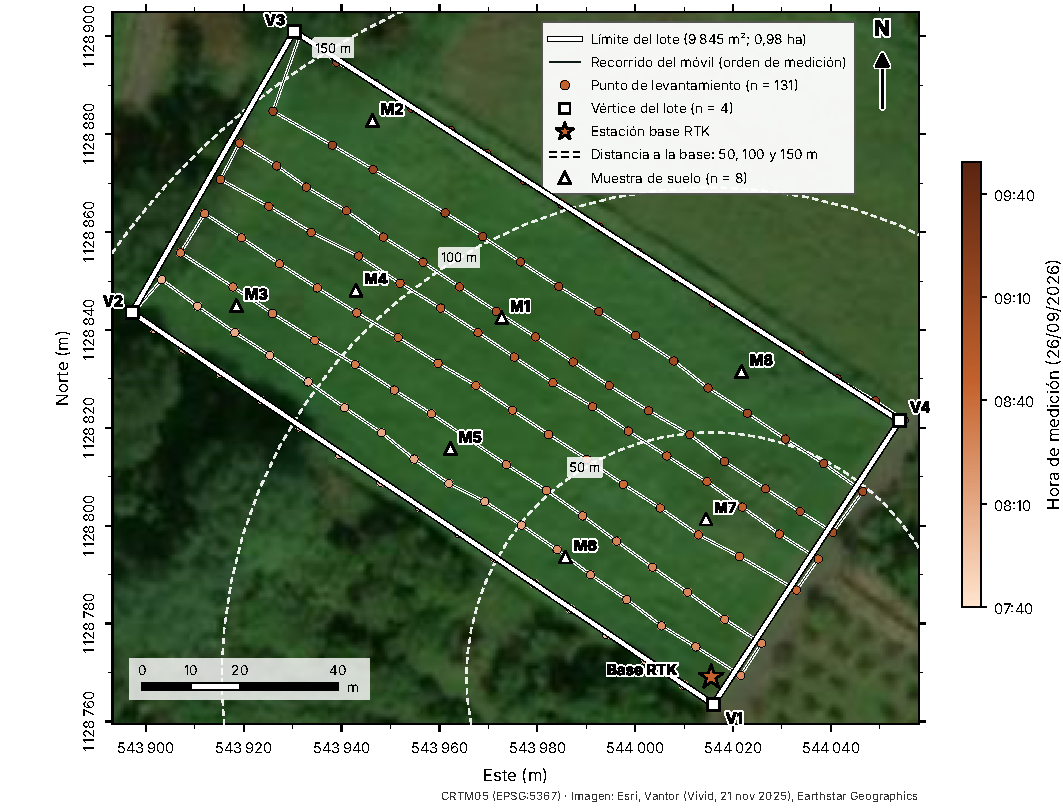
\includegraphics[width=0.9\linewidth]{Figura_Levantamiento.pdf}
\caption{Diseño del levantamiento: estación base, recorrido del móvil en transectos (color según la hora de medición),
vértices y muestras de suelo. Los círculos discontinuos marcan la distancia a la base (línea base RTK).}
\label{fig:levantamiento}
\end{figure}

\subtema{Principio de medición}
El RTK calcula la posición del móvil respecto de la base con la fase de la onda portadora de los satélites. Al restar
las observaciones de dos receptores (A, la base; B, el móvil) a dos satélites (\(j\), \(k\)) se forman
\emph{dobles diferencias}, que eliminan los errores de reloj y, en líneas base cortas, casi todo el efecto de la
ionosfera y de la troposfera (Hofmann-Wellenhof et~al., 2008):
\begin{equation}
  \Phi_{AB}^{jk} = \rho_{AB}^{jk} + \lambda_c\,N_{AB}^{jk} + \varepsilon_{AB}^{jk}
  \label{eq:rtk}
\end{equation}
donde \(\Phi\) es la doble diferencia de fase expresada en metros, \(\rho\) la doble diferencia de las distancias
geométricas entre satélites y receptores, \(\lambda_c\) la longitud de onda de la portadora, \(N\) un número entero de
ciclos (la ambigüedad) y \(\varepsilon\) el ruido de medición. Una \textbf{solución fija} significa que el receptor
resolvió todas las ambigüedades \(N\) como números enteros; solo entonces la posición relativa alcanza precisión
centimétrica. Las líneas base midieron de \BaseMin\ a \BaseMax~m (mediana \BaseMed~m): a esas distancias el error que
crece con la separación, del orden de 1~ppm, es menor de 0,2~mm.

\subtema{Compensación de inclinación}
El bastón no siempre está perfectamente vertical. La unidad inercial (IMU) del receptor mide la inclinación (mediana
\InclMed°, máxima \InclMax°) y traslada la posición del centro de fase de la antena a la punta del bastón:
\begin{equation}
  \mathbf{p}_{\text{punta}} = \mathbf{p}_{\text{antena}} - \mathbf{R}(\phi_r,\theta_r,\psi_r)\,
  \begin{bmatrix} 0 & 0 & h_a \end{bmatrix}^{\mathsf{T}}
  \label{eq:incl}
\end{equation}
donde \(\mathbf{R}\) es la matriz de rotación definida por los ángulos de balanceo, cabeceo y rumbo, y
\mbox{\(h_a = \mnum{\AlturaAnt}\)~m} la altura del centro de fase de la antena sobre la punta del bastón de \Baston~m.

\begin{table}[H]
\caption{Configuración y calidad del levantamiento RTK-GNSS (valores de los \NPuntosTotal\ puntos del Anexo~B).}
\begin{tabularx}{\linewidth}{@{}L{3.9cm}Y@{}}
\toprule
\cab{ELEMENTO} & \cab{VALOR} \\ \midrule
Equipo & Dos receptores GNSS SingularXYZ X1 en modo RTK (base y móvil); correcciones por radio UHF \\ \filete
Satélites & \SatRastMin\ a \SatRastMax\ rastreados; \SatUsoMin\ a \SatUsoMax\ usados en la solución (multiconstelación) \\ \filete
Registro por punto & Punto promediado de \Epocas\ épocas (ocupación típica de \Ocupacion~s); solo solución fija \\ \filete
Bastón y antena & Bastón de \Baston~m; centro de fase a \AlturaAnt~m; inclinación mediana \InclMed°, máxima \InclMax° \\ \filete
Línea base & \BaseMin\ a \BaseMax~m (mediana \BaseMed~m) \\ \filete
Geometría satelital & PDOP \PdopMin\ a \PdopMax; HDOP~≤~\HdopMax; VDOP~≤~\VdopMax \\ \filete
Precisión del receptor (RMS) & Horizontal \mbox{\HrmsMin–\HrmsMax}~cm (mediana \HrmsMed); vertical \mbox{\VrmsMin–\VrmsMax}~cm (mediana \VrmsMed) \\ \filete
Puntos & \NVertices\ vértices, \NElev\ puntos de levantamiento y \NMuestras\ muestras de suelo: \NPuntosTotal\ en total \\ \filete
Jornada & 26 de septiembre de 2026, \HoraInicio\ a \HoraFin\ (\DuracionLev) \\
\bottomrule
\end{tabularx}
\end{table}

% ---------------------------------------------------------------------------- 05.2
\subsection{Sistema de referencia, alturas y área}\label{sec:met-ref}
Todas las coordenadas están en \textbf{CRTM05}, la proyección cartográfica oficial de Costa Rica (Costa Rica, 2007), que se
mantuvo al actualizar el datum a CR-SIRGAS (Costa Rica, 2018). Es una proyección transversa de Mercator con
meridiano central \(L_0 = 84\text{°}\)~O, factor de escala \(k_0 = 0{,}9999\), falso este \mbox{\(x_0 = 500\,000\)~m} y falso
norte \(y_0 = 0\), sobre el elipsoide WGS~84 (\(a = 6\,378\,137\)~m; \(f = 1/298{,}257223563\)); en los mapas se
identifica como EPSG:5367. De latitud \(\varphi\) y longitud \(L\) a Este \(x\) y Norte \(y\) (Snyder, 1987):
\begin{align}
  x &= x_0 + k_0\,R_N\left[A + (1-T+C)\frac{A^3}{6} + (5-18T+T^2+72C-58e'^2)\frac{A^5}{120}\right] \label{eq:tmx}\\
  y &= y_0 + k_0\left\{M(\varphi) + R_N\tan\varphi\left[\frac{A^2}{2} + (5-T+9C+4C^2)\frac{A^4}{24}
       + (61-58T+T^2+600C-330e'^2)\frac{A^6}{720}\right]\right\} \label{eq:tmy}
\end{align}
con \(R_N = a/\sqrt{1-e^2\sin^2\varphi}\) el radio de curvatura del primer vertical, \(T = \tan^2\varphi\), \(C = e'^2\cos^2\varphi\),
\(A = (L-L_0)\cos\varphi\), \(e^2 = f(2-f)\), \(e'^2 = e^2/(1-e^2)\) y \(M(\varphi)\) la longitud del arco de meridiano
desde el ecuador. Usamos la transformación inversa para dar latitud y longitud en el Anexo~B y para reproyectar la
imagen satelital (Sección~\ref{sec:met-carto}). Como la base se posicionó de forma autónoma, la posición absoluta de
todo el levantamiento tiene una incertidumbre de algunos metros; la diferencia entre realizaciones del marco
(CR05, CR-SIRGAS o WGS~84, del orden de decímetros) es menor que esa incertidumbre. Las distancias, las áreas y las
diferencias de altura dentro del lote, que son las que usan todos los mapas, conservan la precisión centimétrica.

\subtema{Alturas}
El receptor entrega alturas elipsoidales \(h\) (WGS~84). La elevación sobre el nivel del mar \(H\) se aproxima restando
la ondulación del geoide \(N\):
\begin{equation}
  H \approx h - N, \qquad N_{\text{EGM2008}} = \mnum{\Geoide}~\text{m}
  \label{eq:geoide}
\end{equation}
\(N\) se obtuvo del modelo EGM2008 (Pavlis et~al., 2012) en el centroide del lote con GeoidEval (Karney, 2026), por
interpolación en la malla del modelo (error RMS ≈ 1~mm). Dentro de un lote de unos 160~m el geoide cambia muy poco, por lo
que se usó un valor constante. Estas alturas son ortométricas aproximadas referidas a EGM2008, no al datum vertical
oficial de Costa Rica (nivelación referida al nivel medio del mar), y heredan la incertidumbre absoluta de la base; las
diferencias de altura dentro del lote no dependen de \(N\).

\subtema{Área y perímetro}
El área del polígono de vértices \((x_i, y_i)\), con \(i = 1,\dots,4\) y \((x_5, y_5) = (x_1, y_1)\), se calculó con
la fórmula del área de Gauss y el perímetro con la suma de los lados:
\begin{equation}
  A_{\text{lote}} = \frac{1}{2}\left|\sum_{i=1}^{4}\left(x_i\,y_{i+1} - x_{i+1}\,y_i\right)\right|, \qquad
  P = \sum_{i=1}^{4}\sqrt{(x_{i+1}-x_i)^2 + (y_{i+1}-y_i)^2}
  \label{eq:area}
\end{equation}
Los resultados, \AreaLote~m² de área y \Perimetro~m de perímetro, son valores de cuadrícula CRTM05; por el factor de
escala de la proyección en el lote (\(k \approx 0{,}99992\)), el área sobre el terreno es ≈\,1,5~m² mayor (0,015~\%).

% ---------------------------------------------------------------------------- 05.3
\subsection{Modelo digital de elevación: spline de placa delgada}\label{sec:met-mde}
Los mapas necesitan una superficie continua, pero medimos puntos aislados. Con los \NElev\ puntos de levantamiento y las
\NMuestras\ muestras (\(n = \NPuntos\); los vértices solo definen el límite) interpolamos la elevación con un
\textbf{spline de placa delgada} (\emph{thin-plate spline}, TPS) y la evaluamos en una malla de 0,25~m
(\MallaFilas\,×\,\MallaCols\ nodos; \MallaCeldas\ dentro del lote). La superficie es
\begin{equation}
  f(x,y) = a_0 + a_1x + a_2y + \sum_{i=1}^{n} w_i\,\phi\!\left(r_i\right), \qquad
  \phi(r) = r^2\ln r, \qquad r_i = \left\lVert (x,y) - (x_i,y_i)\right\rVert
  \label{eq:tps}
\end{equation}
y sus coeficientes resuelven el sistema lineal
\begin{equation}
  \left(\mathbf{K} + \lambda\,\mathbf{I}\right)\mathbf{w} + \mathbf{P}\,\mathbf{a} = \mathbf{z}, \qquad
  \mathbf{P}^{\mathsf{T}}\mathbf{w} = \mathbf{0}
  \label{eq:tpssis}
\end{equation}
con \(K_{ij} = \phi(\lVert (x_i,y_i)-(x_j,y_j)\rVert)\), \(\mathbf{P}\) la matriz \(n \times 3\) de filas
\([1,\;x_i,\;y_i]\) y \(\mathbf{z}\) el vector de las \(n\) elevaciones medidas. La solución es la función que minimiza
(Duchon, 1977; Wahba, 1990)
\begin{equation}
  \sum_{i=1}^{n}\bigl(z_i - f(x_i,y_i)\bigr)^2 + \lambda'\,J(f), \qquad
  J(f) = \iint_{\mathbb{R}^2}\left(f_{xx}^2 + 2f_{xy}^2 + f_{yy}^2\right)\mathrm{d}x\,\mathrm{d}y
  \label{eq:tpsfun}
\end{equation}
\(J(f)\) es la \emph{energía de flexión} de una placa delgada: la suma, sobre toda la superficie, de los cuadrados de sus segundas derivadas, una medida de cuánto se curva. El
primer término premia el ajuste a los datos y el segundo castiga las ondulaciones; el parámetro de suavizado
\(\lambda\), proporcional a \(\lambda'\), regula el equilibrio. Con \(\lambda = 0\) la superficie pasa exactamente por
todos los puntos; con \(\lambda > 0\) se acerca a ellos sin tocarlos y filtra el ruido vertical del RTK
(RMS ≈ 2~cm) y el microrrelieve del pasto, que no forman parte del terreno. Usamos la implementación
\texttt{RBFInterpolator} de SciPy (Virtanen et~al., 2020), con las coordenadas centradas en la media de los puntos.

\subtema{Elección del suavizado por validación cruzada}
Elegimos \(\lambda\) de forma objetiva, con validación cruzada dejando uno fuera (Stone, 1974): se ajusta la superficie
sin el punto \(i\), se predice su elevación y se repite para los \(n\) puntos:
\begin{equation}
  \mathrm{RMSE}_{\mathrm{CV}}(\lambda) = \sqrt{\frac{1}{n}\sum_{i=1}^{n}
  \Bigl(\hat f_{\lambda}^{(-i)}(x_i,y_i) - z_i\Bigr)^2}, \qquad
  \lambda^{*} = \arg\min_{\lambda}\,\mathrm{RMSE}_{\mathrm{CV}}(\lambda)
  \label{eq:loocv}
\end{equation}
Evaluamos ocho valores de \(\lambda\) entre 0 y 1000 (Tabla~\ref{tab:lambda}); el mínimo está en
\(\lambda^{*} = \Suavizado\), con un error de validación de \RMSE~cm. El error de ajuste en los propios puntos es
menor (\RMSEajuste~cm), lo que confirma que la validación cruzada mide la capacidad de predecir y no solo de copiar los
datos.

\begin{table}[H]
\caption{Error de validación cruzada del spline según el parámetro de suavizado \(\lambda\) (\(n = \NPuntos\)).}
\label{tab:lambda}
\small\tnum
\begin{tabular*}{\linewidth}{@{\extracolsep{\fill}}lrrrr@{}}
\toprule
\cab{\(\lambda\)} & \cab{RMSE (cm)} & \cab{MAE (cm)} & \cab{P90 |ERROR| (cm)} & \cab{≤ 12,5 cm} \\ \midrule
0 & 8,48 & 6,23 & 12,7 & 89,9~\% \\ \filete
1 & 8,45 & 6,21 & 12,7 & 89,2~\% \\ \filete
3 & 8,39 & 6,17 & 12,7 & 89,2~\% \\ \filete
10 & 8,27 & 6,09 & 12,5 & 90,6~\% \\ \filete
30 & 8,09 & 6,00 & 12,2 & 91,4~\% \\ \filete
\semi 100 & 7,97 & 6,04 & 12,2 & 91,4~\% \\ \filete
300 & 8,09 & 6,30 & 12,2 & 90,6~\% \\ \filete
1000 & 8,54 & 6,77 & 13,4 & 88,5~\% \\
\bottomrule

\end{tabular*}
\end{table}

\begin{figure}[H]
\centering
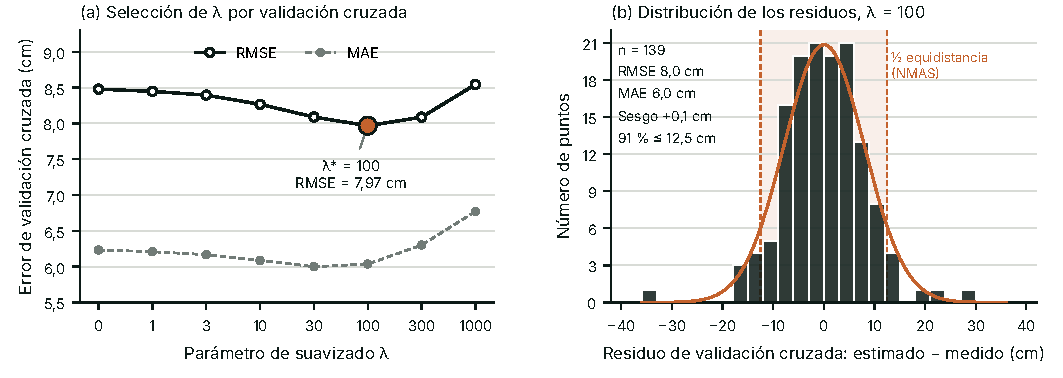
\includegraphics[width=\linewidth]{Figura_Validacion_MDE.pdf}
\caption{Validación del modelo de elevación. (a) Error de validación cruzada según \(\lambda\); el punto de cobre es el
valor elegido. (b) Residuos de validación con \(\lambda = \Suavizado\); la franja marca la tolerancia NMAS para curvas
cada 25~cm (±12,5~cm) y la curva, la distribución normal con la misma media y desviación.}
\label{fig:validacion}
\end{figure}

\subtema{Por qué un spline de placa delgada}
Comparamos el TPS suavizado con cuatro alternativas (el mismo spline sin suavizado, la red de triángulos,
Clough-Tocher y la distancia inversa ponderada) usando la misma validación cruzada (Tabla~\ref{tab:interp}). El TPS
suavizado fue el más exacto y, además, es el más adecuado para derivar pendientes y flujo de agua:

\begin{enumerate}
  \item \textbf{Menor error.} En los \NHull\ puntos donde todos los métodos están definidos, el TPS tuvo un RMSE de
  \RMSETPSHull~cm, frente a \RMSETINHull~cm de la red de triángulos, \RMSECTHull~cm de Clough-Tocher y \RMSEIDWHull~cm
  de la distancia inversa ponderada.
  \item \textbf{Superficie suave, con derivadas continuas.} La pendiente, la dirección de flujo y el TWI dependen de las
  derivadas de la superficie. La red de triángulos produce facetas planas con pendiente discontinua entre ellas, y la
  distancia inversa crea máximos y mínimos locales en cada punto medido, con pendiente nula justo sobre ellos
  (Franke, 1982).
  \item \textbf{Sin semivariograma.} El TPS equivale formalmente a un kriging con tendencia lineal y covarianza
  generalizada \(r^2\ln r\) (Dubrule, 1984), pero no exige estimar un semivariograma ni suponer estacionariedad, que aquí
  no se cumple porque el lote tiene un gradiente general claro (\GradPlano~\%).
  \item \textbf{Cubre todo el lote.} De los \NPuntos\ puntos, \NFuera\ están fuera de la envolvente convexa de los
  demás: allí la red de triángulos y Clough-Tocher no dan valor, mientras que el TPS extrapola de forma suave hasta
  el borde.
  \item \textbf{Respaldo en la literatura.} Las funciones de base radial, familia a la que pertenece el TPS, están
  entre los interpoladores más exactos para modelos de elevación a partir de puntos dispersos (Aguilar et~al., 2005;
  Mitášová y Hofierka, 1993). En Aguilar et~al. (2005) la mejor fue la multicuádrica y el TPS resultó inestable con
  poco suavizado; aquí el suavizado se eligió por validación cruzada (\(\lambda^{*} = \Suavizado\)). Además, el mejor
  método depende del relieve y de la densidad de muestreo, por lo que conviene elegirlo con validación cruzada en los
  propios datos (Chaplot et~al., 2006).
\end{enumerate}

\begin{table}[H]
\caption{Comparación de interpoladores por validación cruzada dejando uno fuera. Las columnas de error usan los
\NHull\ puntos situados dentro de la envolvente convexa de los demás, donde todos los métodos están definidos; la
última columna usa los \NPuntos\ puntos cuando el método lo permite.}
\label{tab:interp}
\tnum
\begin{tabularx}{\linewidth}{@{}Yrrrrr@{}}
\toprule
\cab{MÉTODO} & \cab{RMSE (cm)} & \cab{MAE (cm)} & \cab{SESGO (cm)} & \cab{≤ 12,5 cm} & \cab{RMSE, \(n = \NPuntos\)} \\ \midrule
\semi Spline de placa delgada, $\lambda = 100$ (seleccionado) & 7,6 & 5,8 & −0,2 & 94~\% & 8,0 \\ \filete
Spline de placa delgada, $\lambda = 0$ (interpolación exacta) & 8,2 & 6,1 & −0,1 & 92~\% & 8,5 \\ \filete
Red irregular de triángulos (TIN lineal) & 8,0 & 6,1 & −0,1 & 93~\% & -- \\ \filete
Clough-Tocher (cúbica por triángulos) & 9,2 & 6,8 & −0,5 & 90~\% & -- \\ \filete
Distancia inversa ponderada (IDW, $p = 2$, 12 vecinos) & 9,1 & 7,2 & −0,2 & 84~\% & 9,6 \\
\bottomrule

\end{tabularx}
\end{table}

\subtema{Exactitud y equidistancia de las curvas}
Con \(\lambda = \Suavizado\), la validación cruzada da RMSE~=~\RMSE~cm, MAE~=~\MAE~cm y sesgo \Sesgo~cm; el
percentil~90 del error absoluto es \PNoventa~cm. El estándar NMAS (U.S. Bureau of the Budget, 1947) exige que el
90~\% de los puntos de control tenga un error vertical no mayor que la mitad de la equidistancia. Con curvas cada
25~cm (tolerancia de 12,5~cm) el \NMASpct~\% de los puntos cumple, así que el criterio se satisface; con curvas cada
20~cm no se cumpliría, porque la equidistancia mínima es el doble del percentil~90, unos 24~cm. La exactitud vertical
al 95~\% según el estándar NSSDA (FGDC, 1998), suponiendo errores normales, es
\begin{equation}
  \mathrm{Exactitud}_{z,\,95\%} = 1{,}9600 \times \mathrm{RMSE}_z = 1{,}9600 \times \mnum{\RMSEdos}~\text{cm} = \mnum{\NSSDA}~\text{cm}
  \label{eq:nssda}
\end{equation}
El resultado es poco sensible al suavizado: con \(\lambda = 30\) o \(\lambda = 300\) el error de validación sería de
8,1~cm y la pendiente media, de 1,6 o 1,4~\%.

% ---------------------------------------------------------------------------- 05.4
\subsection{Curvas de nivel, pendiente y gradiente general}\label{sec:met-pend}
Las curvas de nivel se trazaron sobre la malla de 0,25~m con el algoritmo de cuadrados marchantes de Matplotlib,
cada 25~cm y con curva índice cada 50~cm. La pendiente de cada nodo es la magnitud del gradiente de la superficie,
calculado con diferencias finitas centradas de segundo orden (\(\Delta = 0{,}25\)~m):
\begin{equation}
  S = 100\sqrt{\left(\frac{\partial z}{\partial x}\right)^2 + \left(\frac{\partial z}{\partial y}\right)^2}~[\%],
  \qquad
  \frac{\partial z}{\partial x} \approx \frac{z_{i,\,j+1} - z_{i,\,j-1}}{2\Delta}, \quad
  \frac{\partial z}{\partial y} \approx \frac{z_{i+1,\,j} - z_{i-1,\,j}}{2\Delta}
  \label{eq:pend}
\end{equation}
Los límites de 0,5; 1; 2 y 5~\% de las clases de pendiente siguen a FAO (2006, cuadro 7), y los de 1,5 y 3~\% los subdividen; las flechas del mapa apuntan en la dirección de máximo descenso,
\(-\nabla z/\lVert\nabla z\rVert\). El \textbf{gradiente general} del lote se obtuvo ajustando por mínimos cuadrados un
plano a los \NPuntos\ puntos:
\begin{equation}
  z = \beta_0 + \beta_1 x + \beta_2 y, \qquad
  G = 100\sqrt{\beta_1^2 + \beta_2^2} = \mnum{\GradPlano}~\%, \qquad
  \theta = \operatorname{atan2}(-\beta_1,\,-\beta_2) = \AzPlano\text{°}
  \label{eq:plano}
\end{equation}
donde \(\theta\) es el azimut de cuadrícula hacia donde desciende el terreno
(\mbox{\(100\,\beta_1 = \mnum{\PlanoBetaUno}~\%\)}, \mbox{\(100\,\beta_2 = \mnum{\PlanoBetaDos}~\%\)}).

% ---------------------------------------------------------------------------- 05.5
\subsection{Hidrología superficial y humedad topográfica}\label{sec:met-hidro}
El análisis del agua se hizo sobre el spline evaluado en una malla de 1~m, en el lote más una franja de 1,5~m alrededor
(donde aún hay puntos medidos), para que el borde del lote no actúe como una salida artificial.

\subtema{Depresiones}
Las depresiones cerradas, donde el agua puede estancarse, se identificaron rellenando la superficie con el algoritmo
Priority-Flood (Barnes et~al., 2014). Se parte del borde del dominio y se avanza hacia adentro con una cola de
prioridad ordenada por elevación; cada celda vecina \(q\) de una celda ya procesada \(q_0\) recibe
\begin{equation}
  \tilde z(q) = \max\bigl\{\, z(q),\; \tilde z(q_0) + \epsilon \,\bigr\}, \qquad \epsilon = 10^{-5}~\text{m}
  \label{eq:pflood}
\end{equation}
El pequeño incremento \(\epsilon\) da a las zonas planas una pendiente mínima para que el agua pueda salir. La
profundidad de llenado \(d = \tilde z - z\) indica almacenamiento en depresiones; se informan las de
\(d \ge 1\)~cm y área de al menos 5~m².

\subtema{Área de aporte}
El agua de cada celda se repartió entre sus vecinas más bajas con el método de dirección de flujo múltiple de Freeman
(1991), proporcional a la pendiente hacia cada una:
\begin{equation}
  f_k = \frac{(\tan\beta_k)^{p}}{\sum_{j\in D}(\tan\beta_j)^{p}}, \qquad
  \tan\beta_k = \frac{\tilde z_0 - \tilde z_k}{L_k}, \qquad p = 1{,}1
  \label{eq:mfd}
\end{equation}
donde \(D\) es el conjunto de vecinas más bajas (de las ocho), \(L_k\) la distancia al centro de la vecina (1 o
\(\sqrt{2}\)~m) y \(f_k\) la fracción que recibe. Procesando las celdas de la más alta a la más baja, el área de aporte
\(A\) de cada celda es su propia área más todo lo que recibe de las celdas situadas aguas arriba.

\subtema{Índice topográfico de humedad}
Con el área de aporte se calculó el índice topográfico de humedad (TWI):
\begin{equation}
  \mathrm{TWI} = \ln\!\left(\frac{a}{\tan\beta}\right), \qquad a = \frac{A}{w}
  \label{eq:twi}
\end{equation}
donde \(a\) es el área de aporte específica (m² por metro de ancho de celda, \(w = 1\)~m) y \(\beta\) la pendiente
local de la superficie sin rellenar, con \(\tan\beta \ge 0{,}001\) para evitar divisiones entre cero en celdas planas
(Beven y Kirkby, 1979; Moore et~al., 1991). Valores altos indican lugares donde el agua se concentra y el suelo tiende
a permanecer húmedo. En los primeros metros pendiente abajo del borde el TWI está subestimado, porque no incluye el
agua que llega desde fuera del lote.

% ---------------------------------------------------------------------------- 05.6
\subsection{Zonas de manejo: c-medias difuso}\label{sec:met-zonas}
Cada celda de 1~m se describió con tres variables del terreno: elevación, pendiente y TWI. La pendiente y el TWI se
suavizaron con un filtro gaussiano (\(\sigma = 2\)~m) para eliminar ruido de celda a celda, y las tres variables se
estandarizaron, \(x' = (x-\bar x)/s\), para que pesaran igual. Las celdas se agruparon con \textbf{\mbox{c-medias} difuso}
(Bezdek, 1981; Bezdek et~al., 1984), que asigna a cada celda \(i\) un grado de pertenencia \(u_{ik}\) a cada zona \(k\)
y minimiza
\begin{equation}
  J_m = \sum_{i=1}^{n}\sum_{k=1}^{c} u_{ik}^{\,m}\,\lVert \mathbf{x}_i - \mathbf{v}_k \rVert^2,
  \qquad \sum_{k=1}^{c} u_{ik} = 1
  \label{eq:fcm}
\end{equation}
actualizando alternadamente los centros \(\mathbf{v}_k\) y las pertenencias hasta la convergencia:
\begin{equation}
  \mathbf{v}_k = \frac{\sum_{i} u_{ik}^{\,m}\,\mathbf{x}_i}{\sum_{i} u_{ik}^{\,m}}, \qquad
  u_{ik} = \left[\sum_{j=1}^{c}\left(\frac{\lVert \mathbf{x}_i - \mathbf{v}_k\rVert}{\lVert \mathbf{x}_i - \mathbf{v}_j\rVert}\right)^{\frac{2}{m-1}}\right]^{-1}
  \label{eq:fcmupd}
\end{equation}
Usamos distancia euclidiana, exponente de difusividad \(m = 1{,}3\) (el valor por defecto del programa Management Zone Analyst, MZA; Fridgen et~al.,
2004), tolerancia de \(10^{-6}\) y diez inicios aleatorios con semilla fija, conservando la solución de menor \(J_m\).

\subtema{Número de zonas}
Probamos de 2 a 6 zonas y elegimos el número con dos índices de validez (Odeh et~al., 1992; Fridgen et~al., 2004): el
índice de desempeño de la difusividad (FPI) y la entropía de clasificación normalizada (NCE). Ambos miden cuánta
superposición queda entre zonas; cuanto más bajos, mejor definida está la partición:
\begin{equation}
  \mathrm{FPI} = 1 - \frac{c\,F - 1}{c - 1}, \quad F = \frac{1}{n}\sum_{i}\sum_{k} u_{ik}^2; \qquad
  \mathrm{NCE} = \frac{H_u}{1 - c/n}, \quad H_u = -\frac{1}{n}\sum_{i}\sum_{k} u_{ik}\ln u_{ik}
  \label{eq:fpi}
\end{equation}

\begin{table}[H]
\caption{Índices de validez de la zonificación según el número de zonas \(c\). Ambos son mínimos con dos zonas.}
\label{tab:validez}
\small\tnum
\begin{tabular*}{\linewidth}{@{\extracolsep{\fill}}lrr@{}}
\toprule
\cab{ZONAS (\(c\))} & \cab{FPI} & \cab{NCE} \\ \midrule
\semi 2 & 0,147 & 0,124 \\ \filete
3 & 0,171 & 0,195 \\ \filete
4 & 0,167 & 0,221 \\ \filete
5 & 0,190 & 0,275 \\ \filete
6 & 0,182 & 0,281 \\
\bottomrule

\end{tabular*}
\end{table}

Cada celda se asignó a la zona de mayor pertenencia. El mapa se depuró con dos pasadas de un filtro de mayoría de
5\,×\,5~m y uniendo a la zona vecina dominante los parches menores de 100~m² (alrededor del 1~\% del lote). Las zonas se
numeraron de la más baja (Zona~1) a la más alta. La pertenencia media fue de 0,94 en la Zona~1 y de 0,95 en la
Zona~2; con \(m = 1{,}3\) las pertenencias tienden a valores altos, por lo que la separación entre zonas se juzga mejor
con el FPI (0,147) y la NCE (0,124) de la Tabla~\ref{tab:validez}.

% ---------------------------------------------------------------------------- 05.7
\subsection{Muestreo de suelos}\label{sec:met-suelo}
Los ocho puntos de muestreo (M1 a M8) quedaron cuatro en cada zona de manejo y en lugares representativos de ella:
todos tienen una pertenencia de al menos 0,67 a su zona y ninguno está a menos de 2~m del límite entre zonas. Cada punto se
midió con RTK, de modo que puede volver a encontrarse con precisión centimétrica para las pruebas de campo de la
fase~2. En cada punto se tomaron tres submuestras de 0 a 30~cm con un barreno de tubo (sonda muestreadora con mango en T) y se unieron en una muestra compuesta, a fin de
reunir suficiente suelo para los análisis físico y químico (Tabla~\ref{tab:pasos}, pasos 06 y 07).

Con ocho muestras no es posible estimar un semivariograma confiable: se necesitan al menos 100 datos, y los
semivariogramas calculados con menos de 50 tienen poco valor (Webster y Oliver, 1992). Por eso, en la fase~3 los
mapas de las propiedades del suelo combinarán las medias por zona con una regresión sobre la elevación y el TWI, que
sí conocemos en todo el lote.

% ---------------------------------------------------------------------------- 05.8
\subsection{Imagen satelital y cartografía}\label{sec:met-carto}
La imagen de fondo es Esri World Imagery (Vantor Vivid, adquirida el \FechaImagen), servida en teselas de Web Mercator
(EPSG:3857) con nivel de zoom \ZoomImagen, unos \PixelImagen~m por píxel en esta latitud. Para superponerla a los
datos sin deformaciones, cada píxel de la malla de salida en CRTM05 (0,15~m) se llevó a latitud y longitud con la
inversa de la proyección~\eqref{eq:tmx}–\eqref{eq:tmy}, y de ahí a coordenadas de píxel de Web Mercator:
\begin{equation}
  X = 256\cdot 2^{\ell}\,\frac{L + 180\text{°}}{360\text{°}}, \qquad
  Y = 256\cdot 2^{\ell}\,\frac{1}{2}\left[1 - \frac{\ln\left(\tan\varphi + \sec\varphi\right)}{\pi}\right]
  \label{eq:webmerc}
\end{equation}
donde \(\ell\) es el nivel de zoom; el color se obtuvo por interpolación bilineal. Esri declara una exactitud horizontal
de 5~m para esta imagen, por lo que solo sirve como contexto: todas las mediciones provienen del RTK.

Los mapas se elaboraron con Matplotlib (Hunter, 2007). Los mapas
del lote llevan coordenadas CRTM05 en los ejes cada 20~m, flecha de norte de cuadrícula, barra de escala en metros y
leyenda; los de ubicación (Fig.~01) usan ejes cada 100~km y 500~m.
Las paletas están ordenadas por luminosidad y las de las zonas son aptas para personas con daltonismo (Okabe e Ito,
2008).

Todo el procesamiento lo hicimos en Python, a partir de los datos del levantamiento; con los mismos datos, los
cálculos y los mapas pueden repetirse y dan el mismo resultado. Los datos de campo, el código y los mapas están
disponibles en \url{https://github.com/carlychery2001-png/PrecisionAG_Project}.

% ---------------------------------------------------------------------------- 05.9
\needspace{0.45\textheight}
\subsection{Tecnología utilizada}\label{sec:met-stack}
Estas son las herramientas que usamos, desde la medición en el campo hasta los mapas.

\vspace{10pt}
\subtema{Campo y datos de referencia}\noindent
\begin{minipage}[t]{0.31\linewidth}\pila{
\includegraphics[height=13pt]{Informe_Etapa1/logo/stack/singularxyz-logo_c.png}}{SingularXYZ X1}{RTK-GNSS}{Base y móvil con radio UHF y compensación de inclinación.}\end{minipage}\hfill
\begin{minipage}[t]{0.31\linewidth}\pila{\globoicono}{EGM2008}{GeoidEval 2.5.2}{Ondulación del geoide para pasar a elevación sobre el nivel del mar.}\end{minipage}\hfill
\begin{minipage}[t]{0.31\linewidth}\pila{
\includegraphics[height=19pt]{Informe_Etapa1/logo/stack/esri-logo_c.png}}{World Imagery}{Esri}{Imagen satelital de fondo (Vantor Vivid), reproyectada a CRTM05.}\end{minipage}

\vspace{14pt}
\subtema{Procesamiento}\noindent
\begin{minipage}[t]{0.31\linewidth}\pila{
\includegraphics[height=26pt]{Informe_Etapa1/logo/stack/python-logo-only_c.png}}{Python}{3.13}{Lenguaje de todo el procesamiento, de los datos de campo a los mapas.}\end{minipage}\hfill
\begin{minipage}[t]{0.31\linewidth}\pila{
\includegraphics[height=26pt]{Informe_Etapa1/logo/stack/numpylogoicon_c.png}}{NumPy}{2.5}{Mallas, álgebra lineal y estadística (Harris et~al., 2020); mosaico de imágenes con Pillow~12.3.}\end{minipage}\hfill
\begin{minipage}[t]{0.31\linewidth}\pila{
\includegraphics[height=26pt]{Informe_Etapa1/logo/stack/scipy-logo_c.png}}{SciPy}{1.18}{Spline de placa delgada, filtros y etiquetado de zonas (Virtanen et~al., 2020).}\end{minipage}

\vspace{14pt}
\subtema{Cartografía}\noindent
\begin{minipage}[t]{0.31\linewidth}\pila{
\includegraphics[height=17pt]{Informe_Etapa1/logo/stack/matplotlib-logo-full_c.png}}{Matplotlib}{3.11}{Elaboración de los mapas y las figuras (Hunter, 2007).}\end{minipage}\hspace{0.035\linewidth}%
\begin{minipage}[t]{0.31\linewidth}\pila{
\includegraphics[height=26pt]{Informe_Etapa1/logo/stack/osm-logo_c.png}}{OpenStreetMap}{QR}{Ubicación del lote en el teléfono (Sección~\ref{sec:sitio}).}\end{minipage}


% ============================================================================ 06 ENTREGABLES
\section{Entregables y avance}\label{sec:entregables}

\lede{Once entregables oficiales. En la semana 4 hay dos completos y seis con avance parcial; los demás se
completan antes de la presentación final de la semana 13.}

\vspace{4pt}\noindent
\begin{minipage}[t]{0.225\linewidth}\cifra{11}{}{Entregables}\end{minipage}\hfill
\begin{minipage}[t]{0.225\linewidth}\cifra{2}{}{Completados}\end{minipage}\hfill
\begin{minipage}[t]{0.225\linewidth}\cifra{6}{}{Parciales}\end{minipage}\hfill
\begin{minipage}[t]{0.225\linewidth}\cifra{3}{}{Pendientes}\end{minipage}

\vspace{26pt}
\eyebrow[pizarra]{Avance por entregable}\par\vspace{10pt}
\noindent\begin{tikzpicture}[x=1.475cm]
  \celda{0}{01}{C} \celda{1}{02}{C} \celda{2}{03}{P} \celda{3}{04}{P} \celda{4}{05}{P} \celda{5}{06}{N}
  \celda{6}{07}{N} \celda{7}{08}{N} \celda{8}{09}{P} \celda{9}{10}{P} \celda{10}{11}{P}
\end{tikzpicture}\par\vspace{8pt}
{\marcaC\ \eyebrow[pizarra]{Completado}\qquad\marcaP\ \eyebrow[pizarra]{Parcial}\qquad\marcaN\ \eyebrow[pizarra]{Pendiente}}

\vspace{24pt}
\eyebrow[pizarra]{Lo que falta}\par\vspace{2pt}
\begin{tabularx}{\linewidth}{@{}L{3.1cm}Y@{}}
\arrayrulecolor{linea}\midrule\arrayrulecolor{tinta}
\leavevmode{\monomed\color{cobre}Semanas 4 a 8} & \textbf{Laboratorio.} Resultados de los análisis físico (E03) y químico (E04) de las muestras M1–M8. \\ \filete
\leavevmode{\monomed\color{cobre}Semana 6} & \textbf{Campo.} Humedad (E05), compactación (E06) e infiltración (E07) en los puntos de muestreo. \\ \filete
\leavevmode{\monomed\color{cobre}Semanas 9 a 13} & \textbf{Síntesis.} Estado nutricional (E08), mapas de variabilidad (E09), zonas definitivas (E10), plan de fertilización, encalado, riego y drenaje (E11) y presentación final. \\ \filete
\end{tabularx}

\begin{table}[H]
\caption{Entregables oficiales, estado a la semana 4 y semana de entrega.}
\begin{tabularx}{\linewidth}{@{}L{0.7cm}L{3.55cm}YL{2.45cm}L{1.15cm}@{}}
\toprule
\cab{N.º} & \cab{ENTREGABLE} & \cab{CONTENIDO} & \cab{ESTADO} & \cab{SEMANA} \\ \midrule
\leavevmode{\monomed\color{cobre}01} & \entregable{Mapa del campo}{Field map} & Ubicación, polígono con vértices y área, curvas de nivel cada 25~cm y pendientes (Figs. 01 a 04). & \estC & 4 \\ \filete
\leavevmode{\monomed\color{cobre}02} & \entregable{Mapa de muestreo}{Sampling map} & 8 muestras tomadas el 26 de septiembre (M1–M8), cuatro por zona, con coordenadas RTK (Fig. 07). & \estC & 4 \\ \filete
\leavevmode{\monomed\color{cobre}03} & \entregable{Análisis físico del suelo}{Soil physical analysis} & Hecho: muestras M1–M8 tomadas y en el laboratorio. Falta: textura; densidad aparente y porosidad en 4 puntos. & \estP & 4–8 \\ \filete
\leavevmode{\monomed\color{cobre}04} & \entregable{Análisis químico del suelo}{Soil chemical analysis} & Hecho: muestras M1–M8 en el laboratorio. Falta: pH, acidez, bases, P, micronutrientes, materia orgánica y CICE. & \estP & 4–8 \\ \filete
\leavevmode{\monomed\color{cobre}05} & \entregable{Evaluación de la humedad}{Soil moisture assessment} & Hecho: humedad topográfica y depresión (Fig. 05). Falta: humedad gravimétrica en los 8 puntos. & \estP & 6 \\ \filete
\leavevmode{\monomed\color{cobre}06} & \entregable{Evaluación de la compactación}{Compaction assessment} & Resistencia a la penetración hasta 45~cm en los 8 puntos de muestreo. & \estN & 6 \\ \filete
\leavevmode{\monomed\color{cobre}07} & \entregable{Evaluación de la infiltración}{Infiltration assessment} & Infiltración básica con doble anillo en 4 puntos (2 por zona). & \estN & 6 \\ \filete
\leavevmode{\monomed\color{cobre}08} & \entregable{Estado nutricional}{Nutrient status} & Niveles frente a los valores críticos, relaciones catiónicas y saturación de acidez: base del plan de fertilización y encalado. & \estN & 9–10 \\ \filete
\leavevmode{\monomed\color{cobre}09} & \entregable{Mapas de variabilidad espacial}{Spatial variability maps} & Hecho: elevación, pendiente y humedad topográfica. Falta: un mapa por propiedad del suelo. & \estP & 9–10 \\ \filete
\leavevmode{\monomed\color{cobre}10} & \entregable{Zonas de manejo}{Management zones} & Hecho: dos zonas provisionales por terreno (Fig. 06). Falta: validarlas con los datos de suelo. & \estP & 10–11 \\ \filete
\leavevmode{\monomed\color{cobre}11} & \entregable{Recomendaciones de pre-siembra}{Pre-planting recommendations} & Hecho: recomendaciones preliminares (Sección 04.6). Falta: plan de fertilización, encalado, riego y drenaje por zona. & \estP & 11–12 \\
\bottomrule
\end{tabularx}
\end{table}

% ============================================================================ 07 CRONOGRAMA
\section{Cronograma: semanas 4 a 13}

\lede{Diez semanas, de la semana 4 (actual) a la presentación final de la semana 13. Las barras oscuras son
actividades ya realizadas; la línea de cobre marca la semana actual.}

\begin{figure}[H]
\centering
\begin{ganttchart}[
    hgrid={*1{linea, line width=0.3pt}}, vgrid={*1{linea, line width=0.3pt}},
    x unit=1.0cm, y unit title=0.5cm, y unit chart=0.5cm,
    title/.style={draw=none, fill=none},
    title label font=\monomed\fontsize{6.8}{8}\selectfont\color{tinta},
    group/.append style={fill=cobre, draw=none}, group label font=\monomed\fontsize{6.6}{8}\selectfont\addfontfeature{LetterSpace=10}\color{cobre},
    group peaks height=0, group height=0.14, group top shift=0.4, group label node/.append style={left=6pt},
    bar/.append style={fill=white, draw=tinta, line width=0.5pt}, bar height=0.44, bar top shift=0.28,
    bar label font=\fontsize{8}{10}\selectfont\color{grafito}, bar label node/.append style={left=6pt},
    milestone/.append style={fill=cobre, draw=none}, milestone label font=\semi\fontsize{8}{10}\selectfont\color{tinta}, milestone label node/.append style={left=6pt},
    milestone height=0.46, milestone top shift=0.27,
    today=4, today offset=0.5, today rule/.style={draw=cobre, line width=0.9pt},
    today label={\monomed\fontsize{6.5}{8}\selectfont\color{cobre}HOY}, today label node/.append style={anchor=north},
    progress label text={}, bar incomplete/.append style={fill=white},
    inline=false]{4}{13}
  \gantttitle{S4}{1} \gantttitle{S5}{1} \gantttitle{S6}{1} \gantttitle{S7}{1} \gantttitle{S8}{1}
  \gantttitle{S9}{1} \gantttitle{S10}{1} \gantttitle{S11}{1} \gantttitle{S12}{1} \gantttitle{S13}{1} \\
  \gantttitle{\monoreg\fontsize{6}{7}\selectfont\color{pizarra}21/9}{1} \gantttitle{\monoreg\fontsize{6}{7}\selectfont\color{pizarra}28/9}{1}
  \gantttitle{\monoreg\fontsize{6}{7}\selectfont\color{pizarra}5/10}{1} \gantttitle{\monoreg\fontsize{6}{7}\selectfont\color{pizarra}12/10}{1}
  \gantttitle{\monoreg\fontsize{6}{7}\selectfont\color{pizarra}19/10}{1} \gantttitle{\monoreg\fontsize{6}{7}\selectfont\color{pizarra}26/10}{1}
  \gantttitle{\monoreg\fontsize{6}{7}\selectfont\color{pizarra}2/11}{1} \gantttitle{\monoreg\fontsize{6}{7}\selectfont\color{pizarra}9/11}{1}
  \gantttitle{\monoreg\fontsize{6}{7}\selectfont\color{pizarra}16/11}{1} \gantttitle{\monoreg\fontsize{6}{7}\selectfont\color{pizarra}23/11}{1} \\
  \ganttgroup{FASE 1 · DIAGNÓSTICO}{4}{4} \\
  \ganttbar[bar/.append style={fill=tinta}]{Levantamiento RTK y muestreo M1–M8}{4}{4} \\
  \ganttbar[bar/.append style={fill=tinta}]{E01 Mapa del campo}{4}{4} \\
  \ganttbar[bar/.append style={fill=tinta}]{E02 Mapa de muestreo}{4}{4} \\
  \ganttmilestone{Entrega Etapa 01}{4} \\
  \ganttgroup{FASE 2 · CAMPO Y LABORATORIO}{4}{8} \\
  \ganttbar[bar/.append style={fill=tinta}, progress=20]{E03 Análisis físico (laboratorio)}{4}{8} \\
  \ganttbar[bar/.append style={fill=tinta}, progress=20]{E04 Análisis químico (laboratorio)}{4}{8} \\
  \ganttbar{Preparación de las pruebas de campo}{5}{5} \\
  \ganttbar{E05 Humedad del suelo}{6}{6} \\
  \ganttbar{E06 Compactación}{6}{6} \\
  \ganttbar{E07 Infiltración}{6}{6} \\
  \ganttbar{Base de datos de suelo por zona}{8}{8} \\
  \ganttgroup{FASE 3 · SÍNTESIS}{9}{13} \\
  \ganttbar{E08 Estado nutricional}{9}{10} \\
  \ganttbar{E09 Mapas de variabilidad espacial}{9}{10} \\
  \ganttbar{E10 Zonas de manejo definitivas}{10}{11} \\
  \ganttbar{E11 Plan de pre-siembra por zona}{11}{12} \\
  \ganttbar{Informe final}{12}{12} \\
  \ganttmilestone{Presentación final}{13}
\end{ganttchart}
\caption{Cronograma por semana del curso. La fecha indica el lunes de cada semana (2026); la semana 4 corresponde
al 21–27 de septiembre, cuando se levantó el lote.}
\end{figure}

% ============================================================================ 08 INNOVACIÓN
\section{Innovación}

\lede{Seis aportes que van más allá de un diagnóstico convencional.}

\vspace{6pt}\noindent
\begin{minipage}[t]{0.47\linewidth}\rasgo{Exactitud verificada}{Elegimos el interpolador entre cinco alternativas por validación cruzada; la superficie cumple el estándar NMAS para curvas cada 25~cm y un recálculo independiente confirmó los mapas.}\end{minipage}\hfill
\begin{minipage}[t]{0.47\linewidth}\rasgo{Hidrología del lote}{Además de curvas y pendientes, modelamos el flujo del agua para ubicar los problemas de drenaje antes de sembrar.}\end{minipage}

\vspace{14pt}\noindent
\begin{minipage}[t]{0.47\linewidth}\rasgo{Zonas difusas validadas}{C-medias difuso con índices de validez (FPI y NCE); cada una de las ocho muestras se evalúa según su pertenencia a la zona.}\end{minipage}\hfill
\begin{minipage}[t]{0.47\linewidth}\rasgo{Decisiones por zona}{Las zonas y los análisis se traducen en dosis de fertilizante, cal y agua para cada parte del lote, en lugar de una dosis única.}\end{minipage}

\vspace{14pt}\noindent
\begin{minipage}[t]{0.47\linewidth}\rasgo{Registro completo de puntos}{Las coordenadas y la precisión de los \NPuntosTotal\ puntos quedan en el Anexo~B, para volver con RTK a cualquiera de ellos.}\end{minipage}\hfill
\begin{minipage}[t]{0.47\linewidth}\rasgo{Ubicación con un clic}{El código QR de la Sección~\ref{sec:sitio} abre la ubicación del lote en el teléfono, para llegar al sitio sin indicaciones.}\end{minipage}

% ============================================================================ REFERENCIAS
\section*{Referencias}\phantomsection\addcontentsline{toc}{section}{Referencias}
{\fontsize{8.3}{12.2}\linespread{1}\selectfont
\begin{itemize}[label={}, leftmargin=1.2em, itemindent=-1.2em, itemsep=0.45em]
  \item Aguilar, F.J., Agüera, F., Aguilar, M.A., Carvajal, F., 2005. Effects of terrain morphology, sampling density, and interpolation methods on grid DEM accuracy. \emph{Photogrammetric Engineering \& Remote Sensing} 71, 805–816.
  \item Barnes, R., Lehman, C., Mulla, D., 2014. Priority-flood: An optimal depression-filling and watershed-labeling algorithm for digital elevation models. \emph{Computers \& Geosciences} 62, 117–127.
  \item Bertsch, F., 1998. \emph{La fertilidad de los suelos y su manejo}. Asociación Costarricense de la Ciencia del Suelo, San José.
  \item Beven, K.J., Kirkby, M.J., 1979. A physically based, variable contributing area model of basin hydrology. \emph{Hydrological Sciences Bulletin} 24, 43–69.
  \item Bezdek, J.C., 1981. \emph{Pattern Recognition with Fuzzy Objective Function Algorithms}. Plenum Press, Nueva York.
  \item Bezdek, J.C., Ehrlich, R., Full, W., 1984. FCM: The fuzzy c-means clustering algorithm. \emph{Computers \& Geosciences} 10, 191–203.
  \item Bouyoucos, G.J., 1962. Hydrometer method improved for making particle size analyses of soils. \emph{Agronomy Journal} 54, 464–465.
  \item Chaplot, V., Darboux, F., Bourennane, H., Leguédois, S., Silvera, N., Phachomphon, K., 2006. Accuracy of interpolation techniques for the derivation of digital elevation models in relation to landform types and data density. \emph{Geomorphology} 77, 126–141.
  \item Costa Rica, 2007. Decreto Ejecutivo N.° 33797-MJ-MOPT: declara el CR05 como datum horizontal oficial y la proyección transversal de Mercator para Costa Rica (CRTM05) como proyección cartográfica oficial. \emph{La Gaceta} N.° 108, 6 de junio de 2007. Imprenta Nacional, San José.
  \item Costa Rica, 2018. Decreto Ejecutivo N.° 40962-MJP: actualización del sistema geodésico de referencia horizontal oficial para Costa Rica (CR-SIRGAS). \emph{La Gaceta} N.° 66, 17 de abril de 2018, 3–5. Imprenta Nacional, San José.
  \item Dubrule, O., 1984. Comparing splines and kriging. \emph{Computers \& Geosciences} 10, 327–338.
  \item Duchon, J., 1977. Splines minimizing rotation-invariant semi-norms in Sobolev spaces. En: Schempp, W., Zeller, K. (Eds.), \emph{Constructive Theory of Functions of Several Variables}. Lecture Notes in Mathematics 571. Springer, Berlín, 85–100.
  \item FAO, 2006. \emph{Guidelines for Soil Description}, 4.ª ed. Organización de las Naciones Unidas para la Alimentación y la Agricultura, Roma.
  \item FGDC (Federal Geographic Data Committee), 1998. \emph{Geospatial Positioning Accuracy Standards, Part 3: National Standard for Spatial Data Accuracy} (FGDC-STD-007.3-1998). FGDC, Reston, Virginia.
  \item Franke, R., 1982. Scattered data interpolation: tests of some methods. \emph{Mathematics of Computation} 38, 181–200.
  \item Freeman, T.G., 1991. Calculating catchment area with divergent flow based on a regular grid. \emph{Computers \& Geosciences} 17, 413–422.
  \item Fridgen, J.J., Kitchen, N.R., Sudduth, K.A., Drummond, S.T., Wiebold, W.J., Fraisse, C.W., 2004. Management Zone Analyst (MZA): Software for subfield management zone delineation. \emph{Agronomy Journal} 96, 100–108.
  \item Harris, C.R., Millman, K.J., van der Walt, S.J., et~al., 2020. Array programming with NumPy. \emph{Nature} 585, 357–362.
  \item Hofmann-Wellenhof, B., Lichtenegger, H., Wasle, E., 2008. \emph{GNSS – Global Navigation Satellite Systems: GPS, GLONASS, Galileo, and more}. Springer, Viena.
  \item Hunter, J.D., 2007. Matplotlib: A 2D graphics environment. \emph{Computing in Science \& Engineering} 9, 90–95.
  \item Karney, C.F.F., 2026. \emph{GeoidEval}, GeographicLib 2.5.2 (calculadora en línea). \url{https://geographiclib.sourceforge.io/cgi-bin/GeoidEval} (consultada en septiembre de 2026).
  \item Mitášová, H., Hofierka, J., 1993. Interpolation by regularized spline with tension: II. Application to terrain modeling and surface geometry analysis. \emph{Mathematical Geology} 25, 657–669.
  \item Moore, I.D., Grayson, R.B., Ladson, A.R., 1991. Digital terrain modelling: a review of hydrological, geomorphological, and biological applications. \emph{Hydrological Processes} 5, 3–30.
  \item Odeh, I.O.A., McBratney, A.B., Chittleborough, D.J., 1992. Soil pattern recognition with fuzzy-c-means: Application to classification and soil-landform interrelationships. \emph{Soil Science Society of America Journal} 56, 505–516.
  \item Okabe, M., Ito, K., 2008. Color Universal Design (CUD): How to make figures and presentations that are friendly to Colorblind people. J*Fly. \url{https://jfly.uni-koeln.de/color/}
  \item Pavlis, N.K., Holmes, S.A., Kenyon, S.C., Factor, J.K., 2012. The development and evaluation of the Earth Gravitational Model 2008 (EGM2008). \emph{Journal of Geophysical Research: Solid Earth} 117, B04406.
  \item Snyder, J.P., 1987. \emph{Map Projections: A Working Manual}. U.S. Geological Survey Professional Paper 1395. U.S. Government Printing Office, Washington, D.C.
  \item Stone, M., 1974. Cross-validatory choice and assessment of statistical predictions. \emph{Journal of the Royal Statistical Society, Series B} 36, 111–133.
  \item U.S. Bureau of the Budget, 1947. \emph{United States National Map Accuracy Standards}. U.S. Bureau of the Budget, Washington, D.C.
  \item Virtanen, P., Gommers, R., Oliphant, T.E., et~al., 2020. SciPy 1.0: fundamental algorithms for scientific computing in Python. \emph{Nature Methods} 17, 261–272.
  \item Wahba, G., 1990. \emph{Spline Models for Observational Data}. CBMS-NSF Regional Conference Series in Applied Mathematics 59. SIAM, Filadelfia.
  \item Walkley, A., Black, I.A., 1934. An examination of the Degtjareff method for determining soil organic matter, and a proposed modification of the chromic acid titration method. \emph{Soil Science} 37, 29–38.
  \item Webster, R., Oliver, M.A., 1992. Sample adequately to estimate variograms of soil properties. \emph{Journal of Soil Science} 43, 177–192.
\end{itemize}
\nota{Imágenes satelitales: Esri World Imagery (fuente: Esri, Vantor, Earthstar Geographics y la comunidad de usuarios SIG). Capa de referencia: Esri World Boundaries and Places (fuente: Esri, HERE, Garmin, © colaboradores de OpenStreetMap y la comunidad de usuarios SIG). Logotipo de OpenStreetMap: Ken Vermette, CC BY-SA 3.0.}}

% ============================================================================ ANEXOS
\appendix
\makeatletter\renewcommand{\thesection}{\Alph{section}}\makeatother
\section{Control de calidad}
\begin{itemize}
  \item \textbf{Calidad RTK.} Los \NPuntosTotal\ puntos RTK-GNSS del registro (Anexo~B) tienen solución fija: RMS horizontal de \mbox{\HrmsMin–\HrmsMax}~cm, RMS vertical de \mbox{\VrmsMin–\VrmsMax}~cm y PDOP~≤~\PdopMax\ (Sección~\ref{sec:met-campo}).
  \item \textbf{Alturas.} El colector entrega alturas elipsoidales WGS~84; se restó la ondulación del geoide EGM2008 (\Geoide~m). Como la base se posicionó de forma autónoma, la elevación y las coordenadas absolutas tienen una incertidumbre de algunos metros; las diferencias dentro del lote (curvas, pendientes y zonas) no se ven afectadas.
  \item \textbf{Validación de la superficie.} Validación cruzada dejando uno fuera: RMSE de \RMSE~cm; el \NMASpct~\% de los errores queda dentro de la mitad de la equidistancia de 25~cm (estándar NMAS; Sección~\ref{sec:met-mde}).
\end{itemize}


% ============================================================================ ANEXO B · PUNTOS LEVANTADOS
\clearpage
\section{Puntos levantados}\label{sec:puntos}

\lede{Registro de los \NPuntosTotal\ puntos RTK-GNSS tomados el 26 de septiembre de 2026, todos con solución fija:
\NVertices\ vértices del lote, \NMuestras\ muestras de suelo y \NElev\ puntos de levantamiento.}

\nota{Coordenadas en CRTM05 (EPSG:5367) y WGS~84; elevación aproximada sobre el nivel del mar (EGM2008).
RMS~H y RMS~V: precisión horizontal y vertical de cada punto según el receptor; todas las soluciones son fijas.
El archivo completo del levantamiento está en \url{https://github.com/carlychery2001-png/PrecisionAG_Project}.}

\begingroup
\fontsize{7.9}{10.6}\linespread{1}\selectfont\tnum
\setlength{\LTleft}{0pt}\setlength{\LTright}{0pt}\setlength{\LTpre}{0pt}\setlength{\LTpost}{0pt}
\setlength{\tabcolsep}{5pt}\renewcommand{\arraystretch}{1.04}
\CatchFileDef{\filaspuntos}{datos/puntos.tex}{}
\vspace{12pt}\noindent\captionof{table}{Coordenadas, elevación y precisión de los \NPuntosTotal\ puntos levantados.}\label{tab:puntos}\edef\tablapuntos{\thetable}
\begin{longtable}{@{\extracolsep{\fill}}>{\medium\color{tinta}}lrrrrrrr@{}}
\toprule
\cab{PUNTO} & \cab{ESTE (m)} & \cab{NORTE (m)} & \cab{LATITUD} & \cab{LONGITUD} & \cab{ELEV. (m)} & \cab{RMS H (cm)} & \cab{RMS V (cm)} \\ \midrule
\endfirsthead
\multicolumn{8}{@{}l}{\eyebrow{Tabla \tablapuntos\ · continuación}} \\[5pt]
\toprule
\cab{PUNTO} & \cab{ESTE (m)} & \cab{NORTE (m)} & \cab{LATITUD} & \cab{LONGITUD} & \cab{ELEV. (m)} & \cab{RMS H (cm)} & \cab{RMS V (cm)} \\ \midrule\addlinespace[2pt]
\endhead
\bottomrule
\endfoot
\bottomrule
\endlastfoot
\filaspuntos
\end{longtable}
\endgroup

% ============================================================================ ANEXO C · REGISTRO FOTOGRÁFICO
\clearpage
\section{Registro fotográfico}\label{sec:fotos}

\lede{El equipo de trabajo en el lote, con los receptores GNSS del levantamiento.}

\begin{figure}[H]
\centering
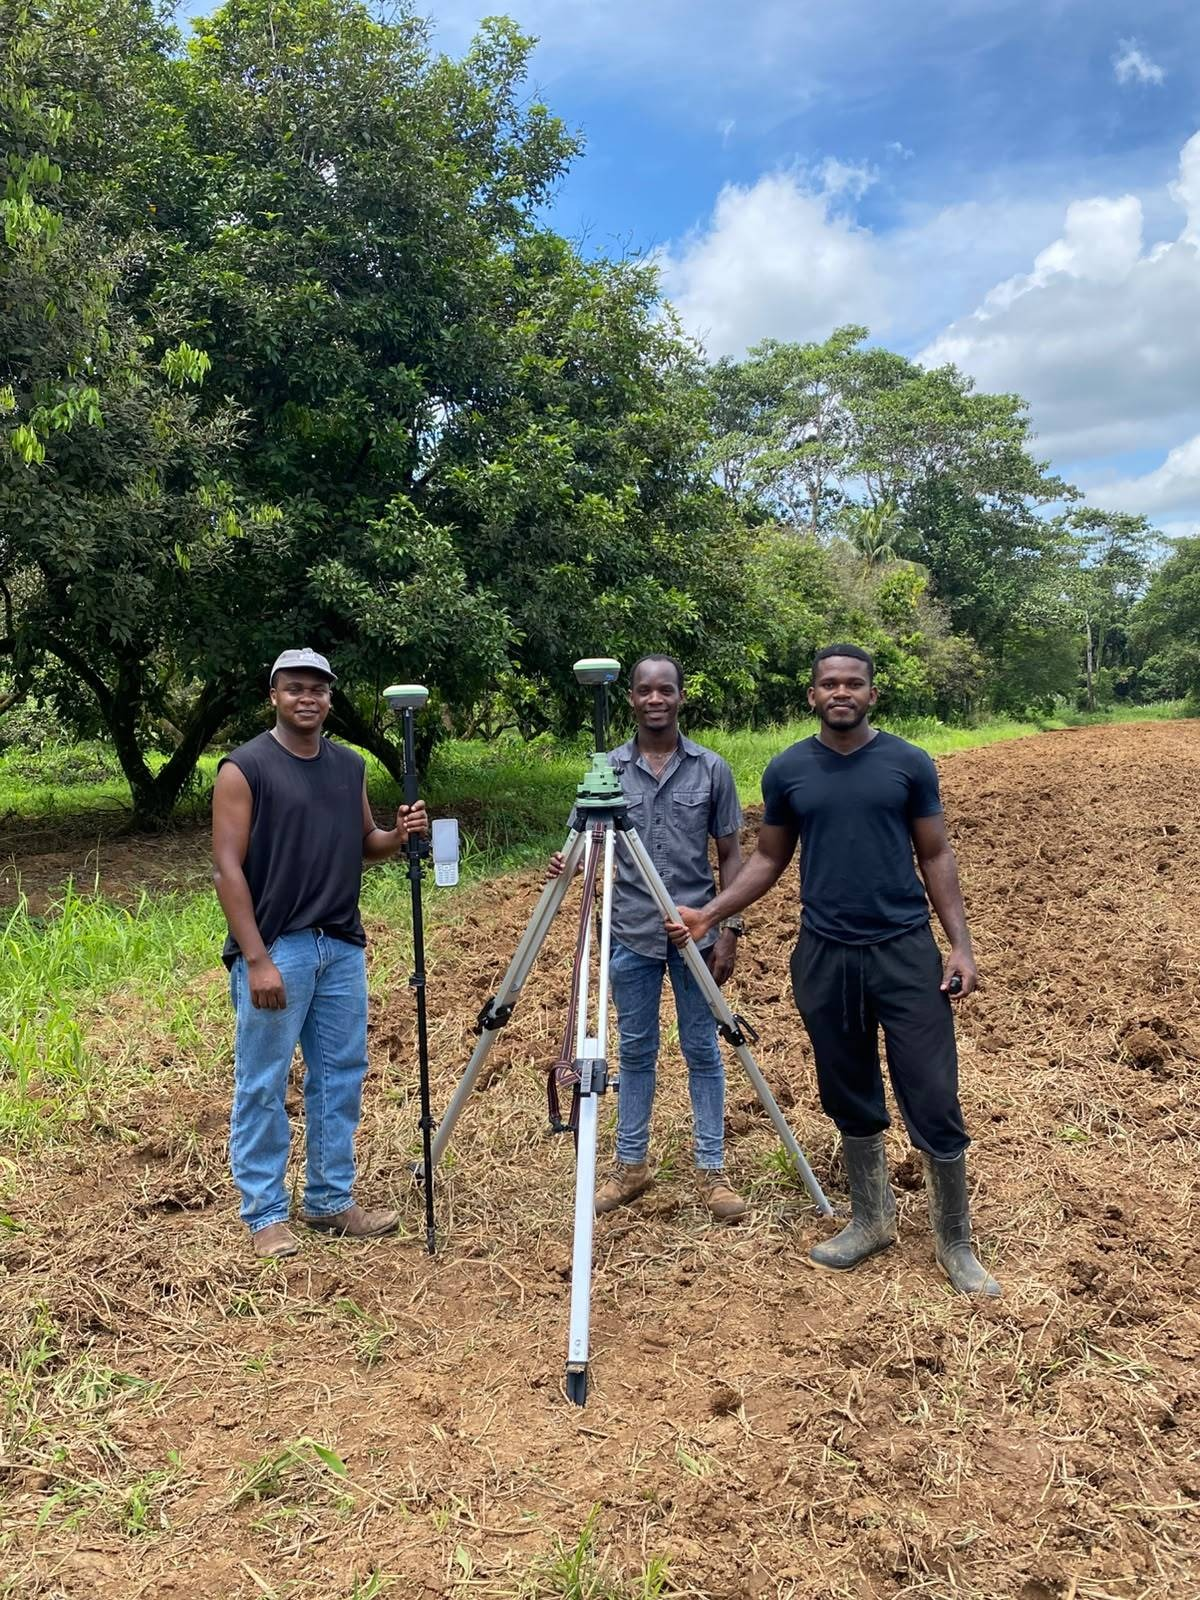
\includegraphics[width=0.62\linewidth]{Informe_Etapa1/fotos/equipo_campo.jpg}
\caption{Levantamiento RTK-GNSS en el lote: la estación base SingularXYZ X1 sobre el trípode y el receptor móvil en el bastón, con el colector de datos.}
\label{fig:equipo}
\end{figure}

\clearpage
\begin{figure}[H]
\centering
\begin{minipage}[t]{0.42\linewidth}
  \centering
  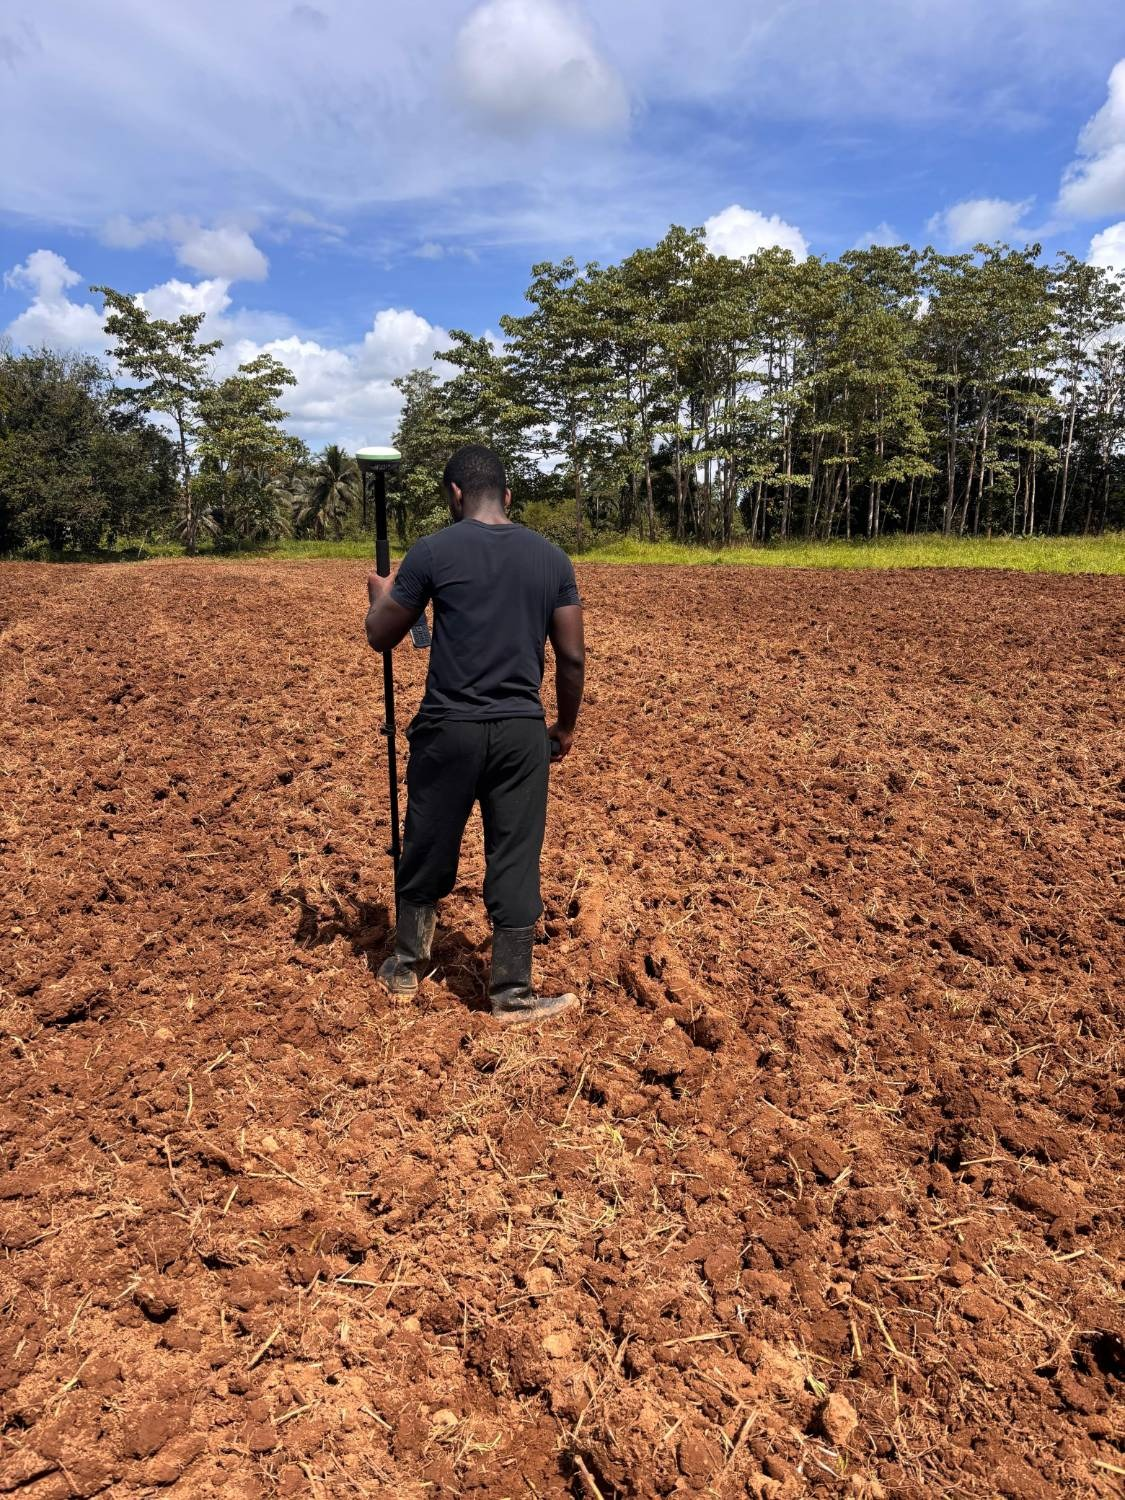
\includegraphics[width=\linewidth]{Informe_Etapa1/fotos/levantamiento_movil.jpg}
  \caption{Carly Chery con el receptor móvil SingularXYZ X1 en el bastón y el colector de datos, durante el levantamiento.}
  \label{fig:movil}
\end{minipage}\hspace{0.06\linewidth}%
\begin{minipage}[t]{0.42\linewidth}
  \centering
  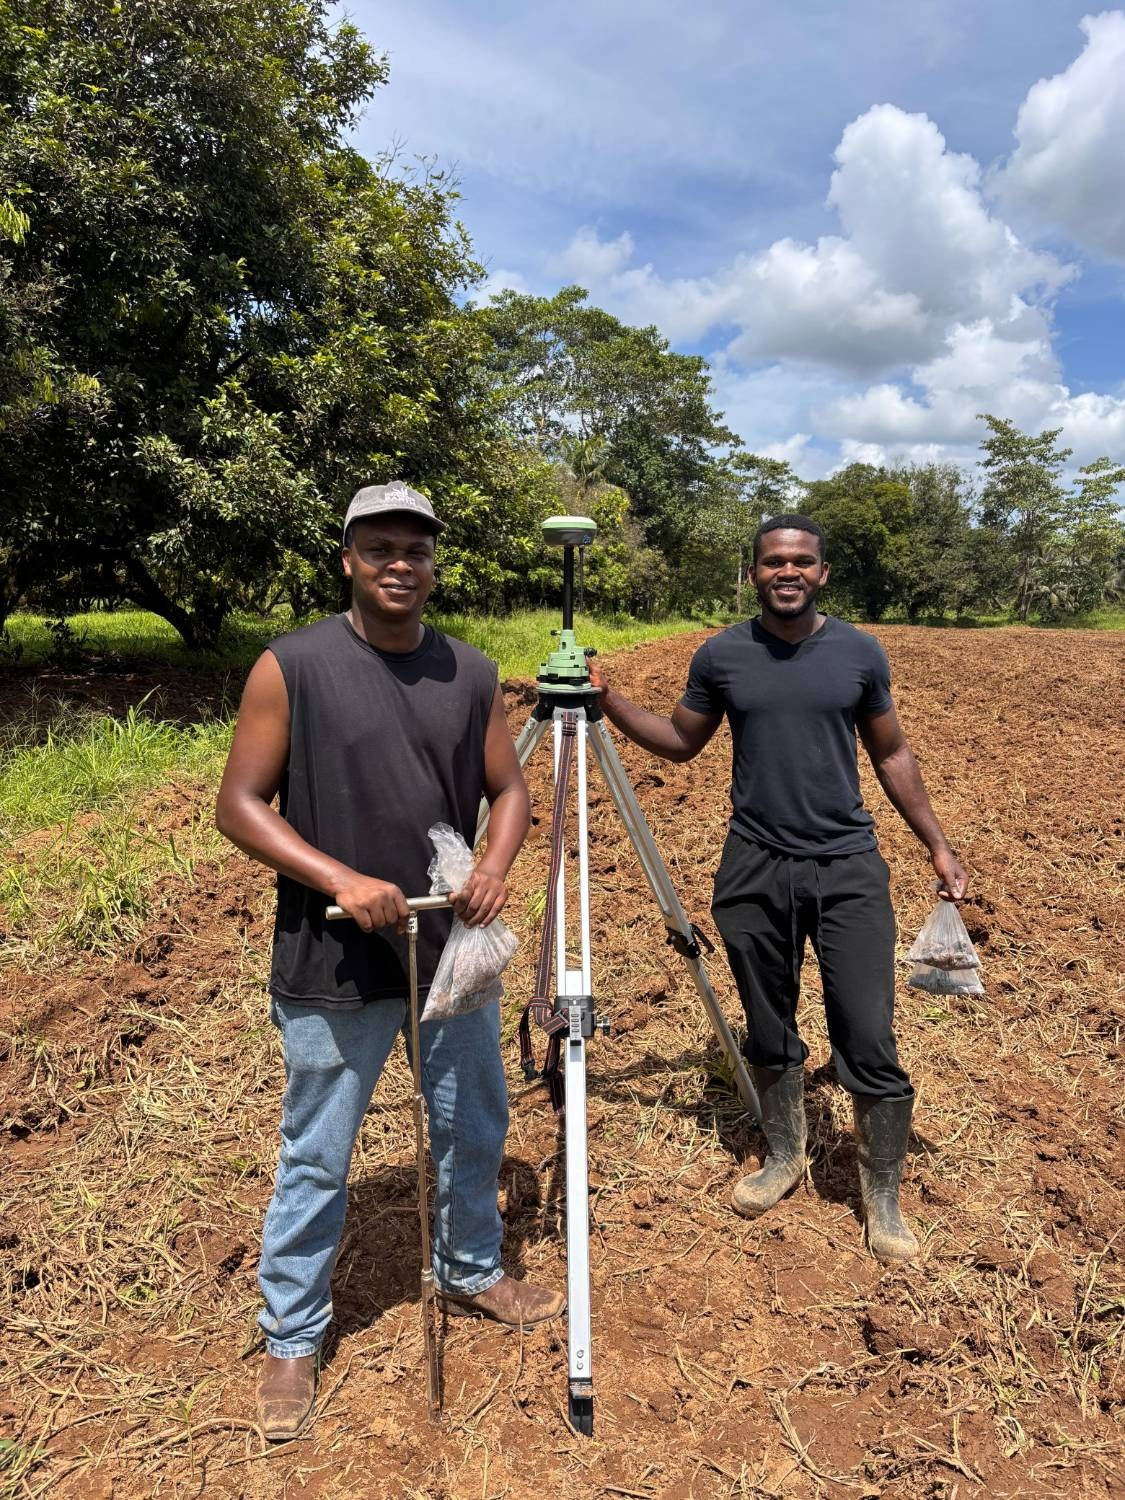
\includegraphics[width=\linewidth]{Informe_Etapa1/fotos/muestreo_barreno.jpg}
  \caption{Muestreo de suelos: Felix Wanjiku con el barreno de tubo y Carly Chery con las muestras compuestas, junto a la estación base.}
  \label{fig:barreno}
\end{minipage}

\vspace{14pt}
\begin{minipage}[t]{0.42\linewidth}
  \centering
  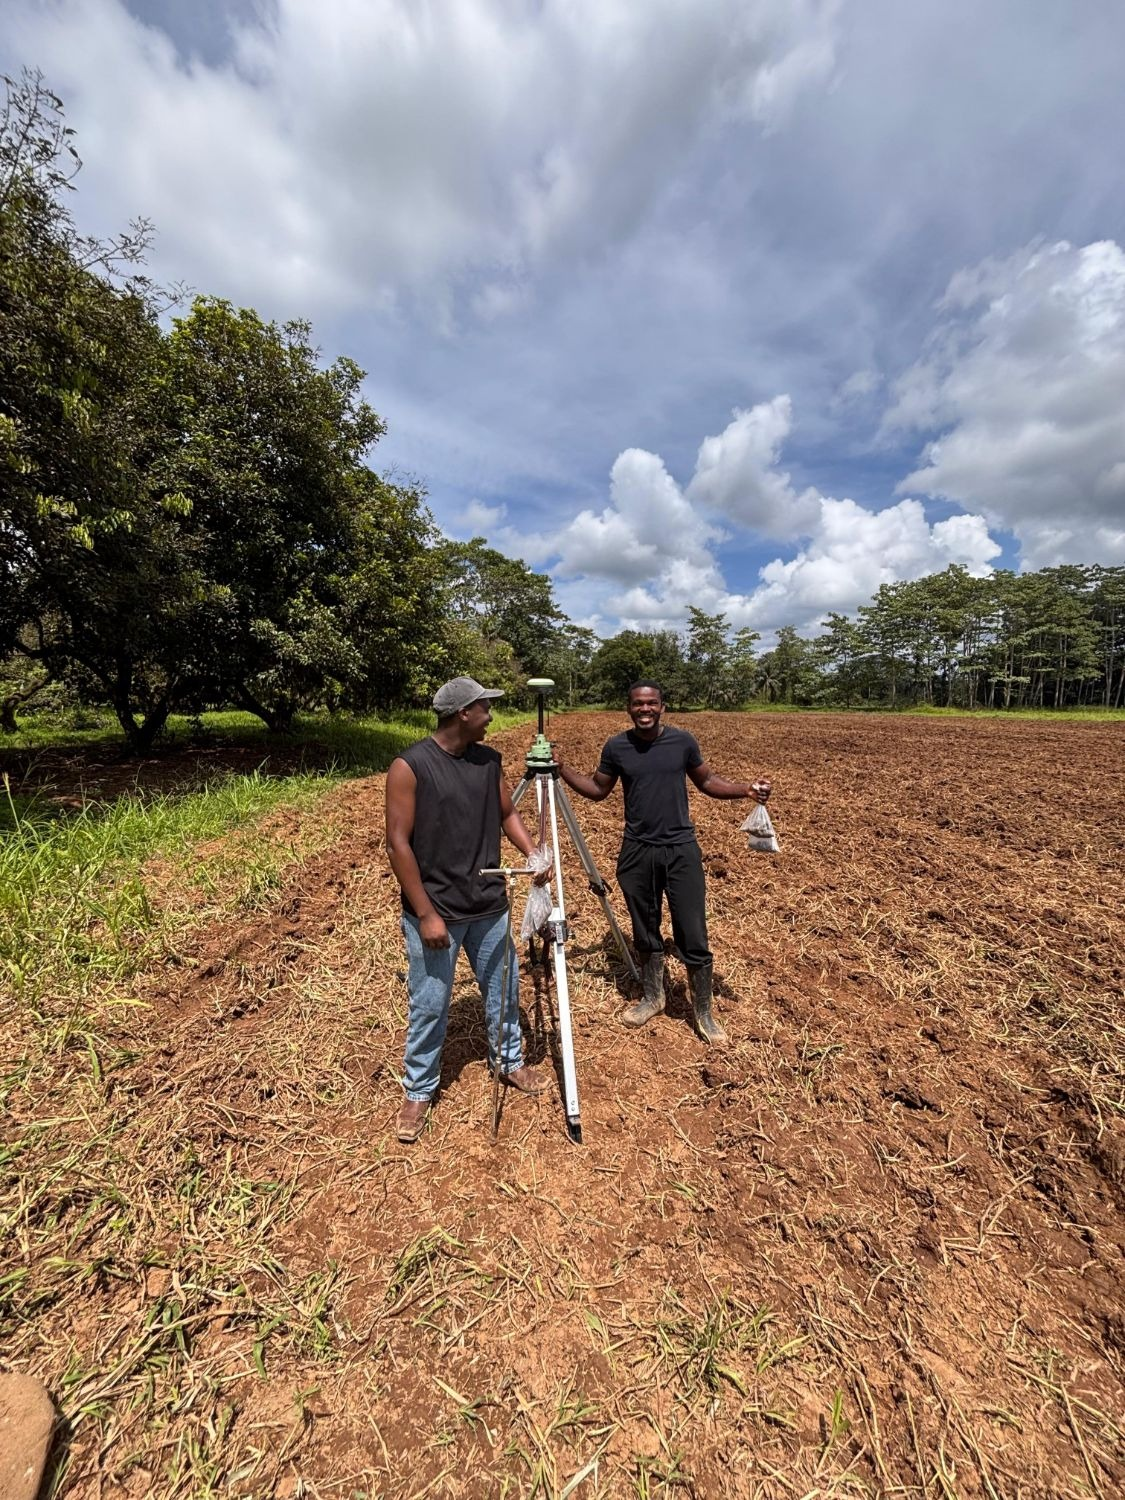
\includegraphics[width=\linewidth]{Informe_Etapa1/fotos/muestreo_base.jpg}
  \caption{Toma de muestras en el lote: Felix Wanjiku con el barreno y una bolsa de muestra, y Carly Chery con las muestras del punto, junto a la estación base.}
  \label{fig:muestreo}
\end{minipage}
\end{figure}

% ============================================================================ CONTRAPORTADA
\clearpage
\thispagestyle{empty}
\begin{tikzpicture}[remember picture, overlay]
  \fill[tinta] (current page.south west) rectangle (current page.north east);
  \node[inner sep=0pt, opacity=0.9] at ([yshift=2.2cm]current page.center)
    {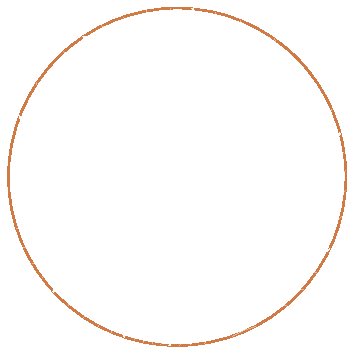
\includegraphics[width=6.2cm]{Informe_Etapa1/arte/sello_curvas.pdf}};
  \node[inner sep=0pt] at ([yshift=-3.4cm]current page.center) {\CotaliaLogo{0.72}{white}{cobre}};
  \node[inner sep=0pt, align=center] at ([yshift=-5.2cm]current page.center)
    {\eyebrow[cobreclaro]{Agricultura de precisión para un manejo eficiente}};
  \node[anchor=south, inner sep=0pt, align=center, text width=15cm] at ([yshift=2.4cm]current page.south)
    {{\monoreg\fontsize{8}{12}\selectfont\color{white}\Correo \quad·\quad \Web}\\[4pt]
     {\fontsize{8}{12}\selectfont\color{white!60!tinta}\Direccion}};
\end{tikzpicture}

\end{document}
